\chapter{Evaluation} \label{section:evaluation} 


\section{MaFaulDa and k-nearest neighbors}

\subsection{Complete feature sets}
% Confusion matrix
\begin{figure}[h]
    \centering
    \begin{subfigure}[b]{0.49\textwidth}
        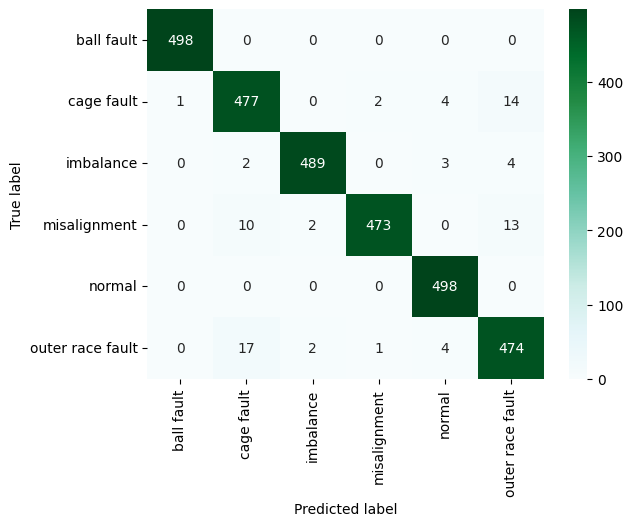
\includegraphics[width=\textwidth]{assets/results/all-features/TD-confusion-matrix.png}
        \caption{Time-domain features}
    \end{subfigure}
    \hfill
    \begin{subfigure}[b]{0.49\textwidth}
        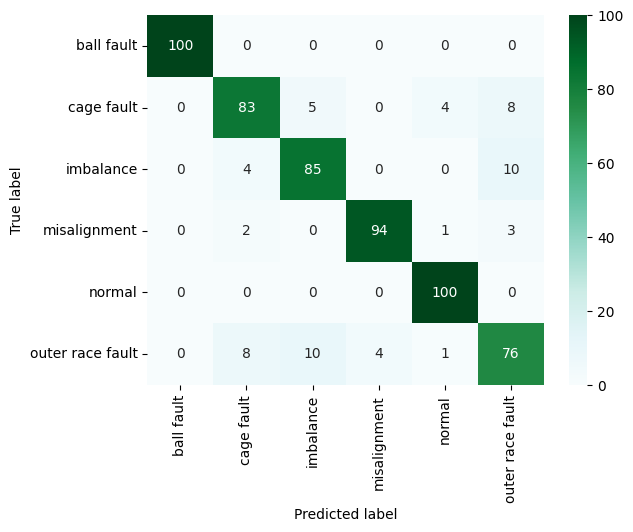
\includegraphics[width=\textwidth]{assets/results/all-features/FD-confusion-matrix.png}
        \caption{Frequency-domain features}
    \end{subfigure}
    \caption{Confusion matrix for complete sets of features }
\end{figure}

% Nearest neighbors - how many points have neighbourhood of same class A+B
\begin{figure}[h]
    \centering
    \begin{subfigure}[b]{0.49\textwidth}
        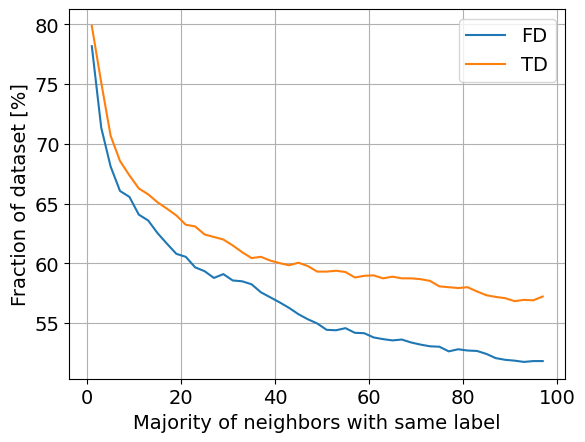
\includegraphics[width=\textwidth]{assets/results/all-features/neighborhood.png}
        \caption{No severity}
    \end{subfigure}
    \hfill
    \begin{subfigure}[b]{0.49\textwidth}
        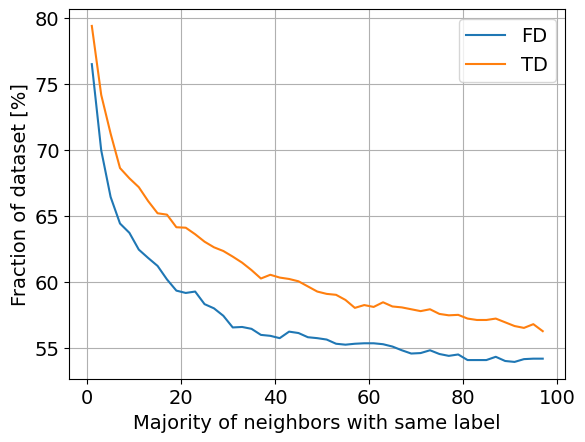
\includegraphics[width=\textwidth]{assets/results/all-features/neighborhood-severity.png}
        \caption{Severity}
    \end{subfigure}
    \caption{Neighborhood with same label}
\end{figure}

% Accuracy based on scenario
% No optimal K - data is noisy
\begin{figure}[h]
    \centering
    \begin{subfigure}[b]{0.48\textwidth}
        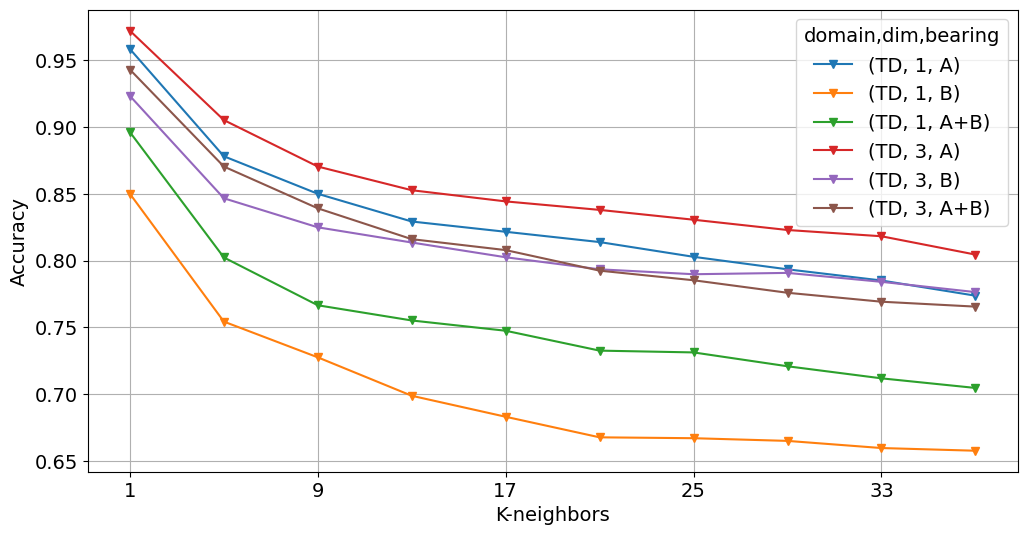
\includegraphics[width=\textwidth]{assets/results/all-features/TD.png}
        \caption{Time-domain features}
    \end{subfigure}
    \hfill
    \begin{subfigure}[b]{0.48\textwidth}
        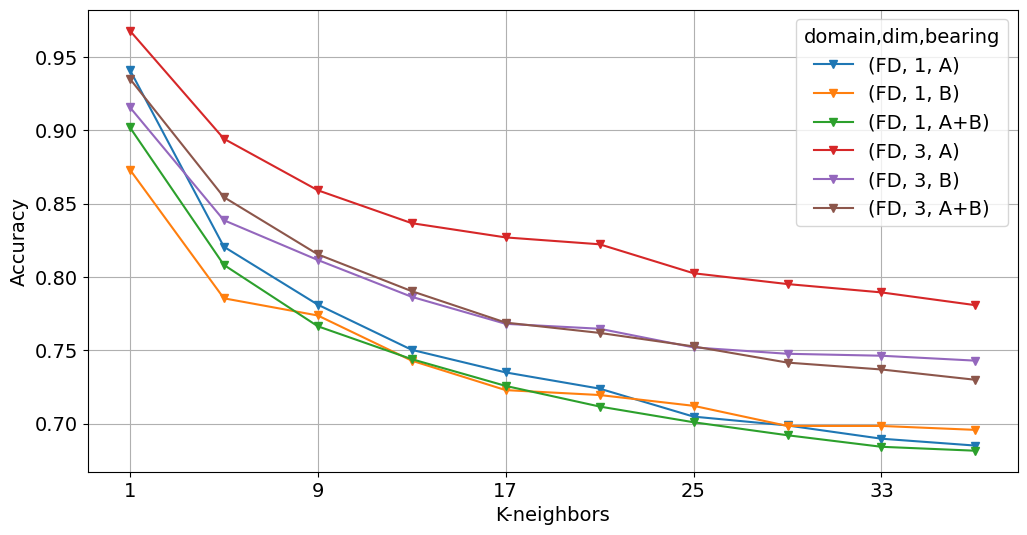
\includegraphics[width=\textwidth]{assets/results/all-features/FD.png}
        \caption{Frequency-domain features}
    \end{subfigure}
    \hfill
    \begin{subfigure}[b]{0.48\textwidth}
        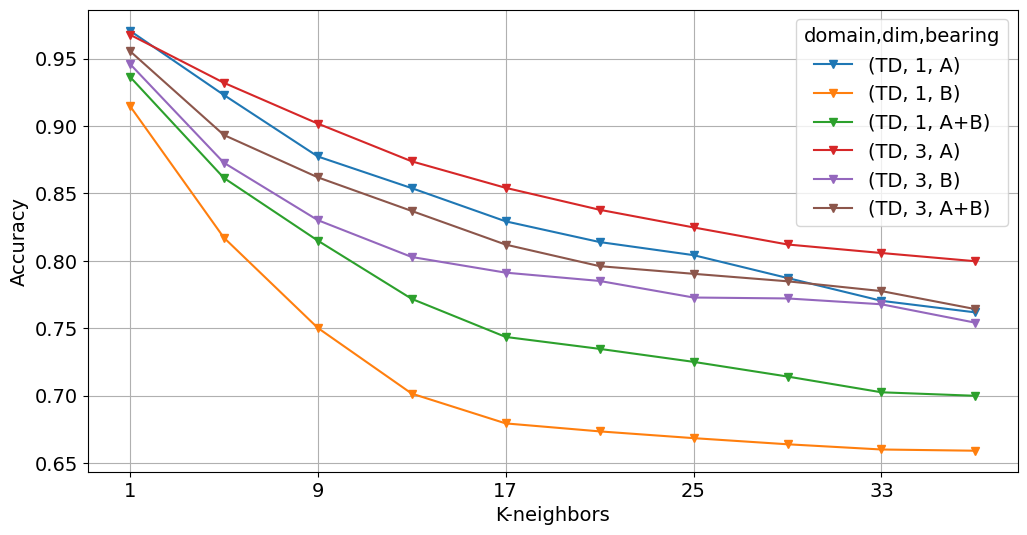
\includegraphics[width=\textwidth]{assets/results/all-features/TD-severity.png}
        \caption{Time-domain features (severity)}
    \end{subfigure}
    \hfill
    \begin{subfigure}[b]{0.48\textwidth}
        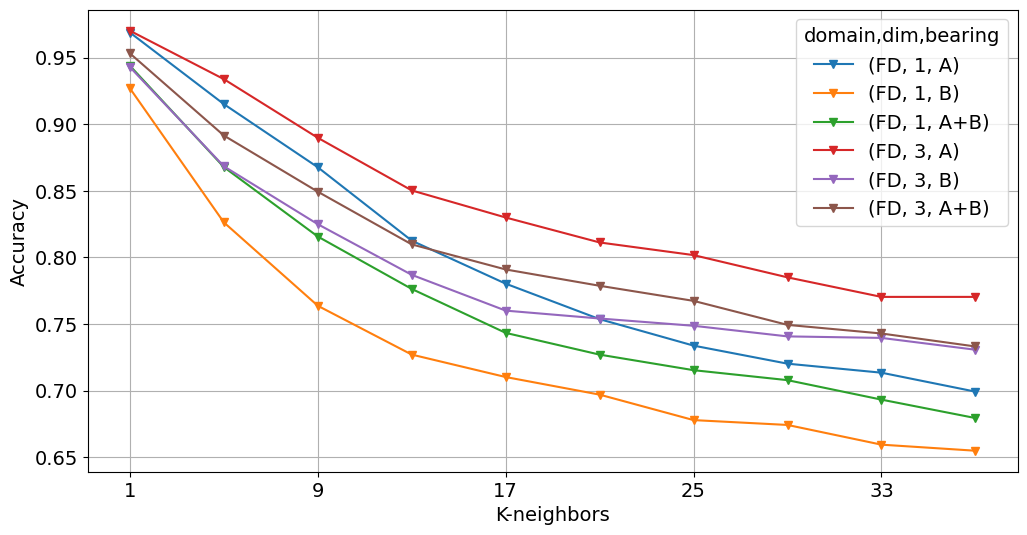
\includegraphics[width=\textwidth]{assets/results/all-features/FD-severity.png}
        \caption{Frequency-domain features (severity)}
    \end{subfigure} 
    \caption{Accuracy dependency on k-value}
\end{figure}


\subsection{Feature subset combinations}
% Boxplots
\begin{figure}[h]
    \centering
    \begin{subfigure}[b]{0.48\textwidth}
        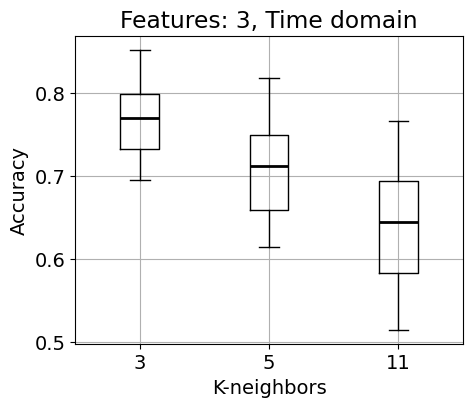
\includegraphics[width=\textwidth]{assets/results/feature-combinations/TD-3-A+B-False-False-F3.png}
        \caption{Time domain features}
    \end{subfigure}
    \hfill
    \begin{subfigure}[b]{0.48\textwidth}
        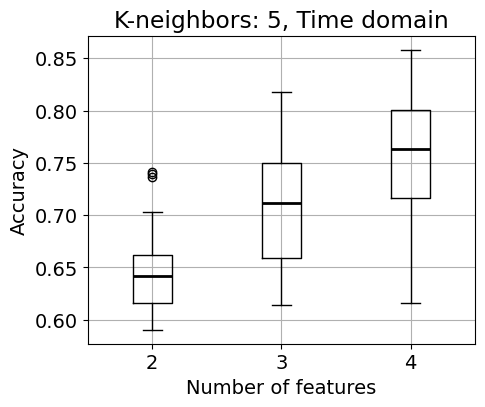
\includegraphics[width=\textwidth]{assets/results/feature-combinations/TD-3-A+B-False-False-K5.png}
        \caption{Time domain features}
    \end{subfigure}
    \hfill
    \begin{subfigure}[b]{0.48\textwidth}
        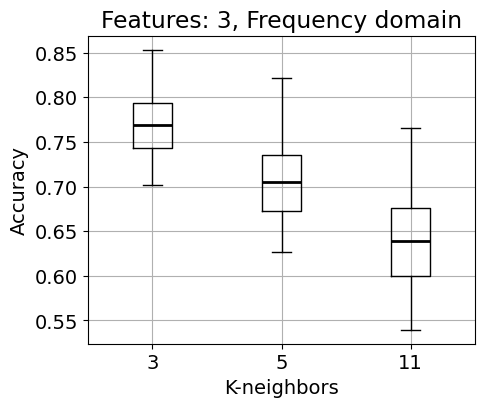
\includegraphics[width=\textwidth]{assets/results/feature-combinations/FD-3-A+B-False-False-F3.png}
        \caption{Frequency domain features}
    \end{subfigure}
    \hfill
    \begin{subfigure}[b]{0.48\textwidth}
        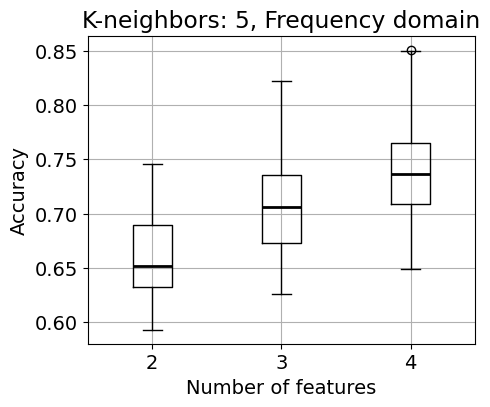
\includegraphics[width=\textwidth]{assets/results/feature-combinations/FD-3-A+B-False-False-K5.png}
        \caption{Frequency domain features}
    \end{subfigure}
    \caption{Model accuracy distribution (Bearings A+B, Dim = 3, Severity False)}
\end{figure}


\begin{figure}[h]
    \centering
    \begin{subfigure}[b]{0.48\textwidth}
        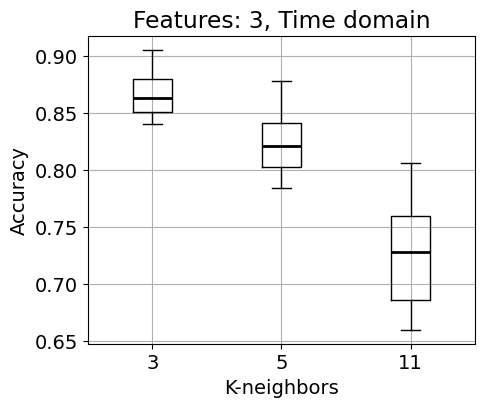
\includegraphics[width=\textwidth]{assets/results/feature-combinations/TD-3-A+B-True-False-F3.png}
        \caption{Time domain features}
    \end{subfigure}
    \hfill
    \begin{subfigure}[b]{0.48\textwidth}
        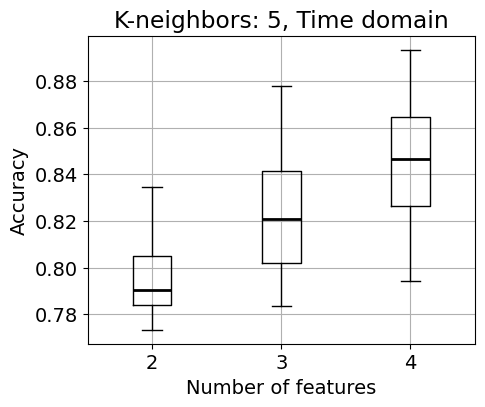
\includegraphics[width=\textwidth]{assets/results/feature-combinations/TD-3-A+B-True-False-K5.png}
        \caption{Time domain features}
    \end{subfigure}
    \hfill
    \begin{subfigure}[b]{0.48\textwidth}
        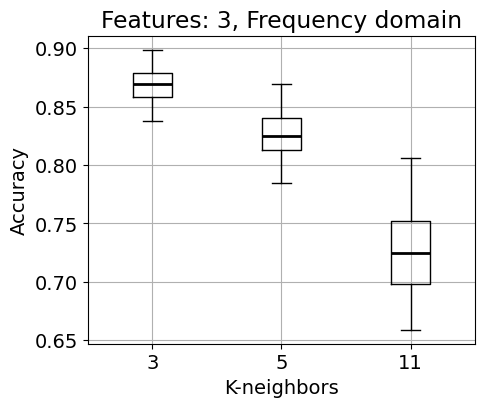
\includegraphics[width=\textwidth]{assets/results/feature-combinations/FD-3-A+B-True-False-F3.png}
        \caption{Frequency domain features}
    \end{subfigure}
    \hfill
    \begin{subfigure}[b]{0.48\textwidth}
        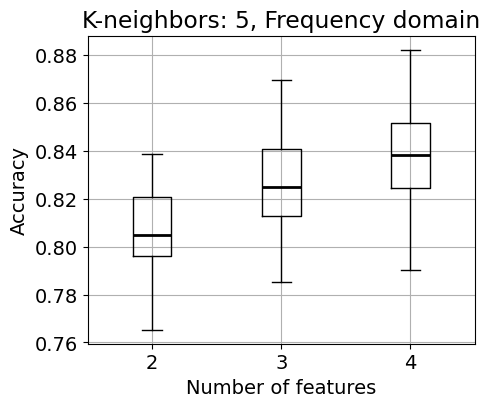
\includegraphics[width=\textwidth]{assets/results/feature-combinations/FD-3-A+B-True-False-K5.png}
        \caption{Frequency domain features}
    \end{subfigure}
    \caption{Model accuracy distribution (Severity True)}
\end{figure}


\subsection{Feature selection techniques}
% Accuracy tables
% Compare linear complexity accuracy with whole distribution
\begin{figure}[h]
    \centering
    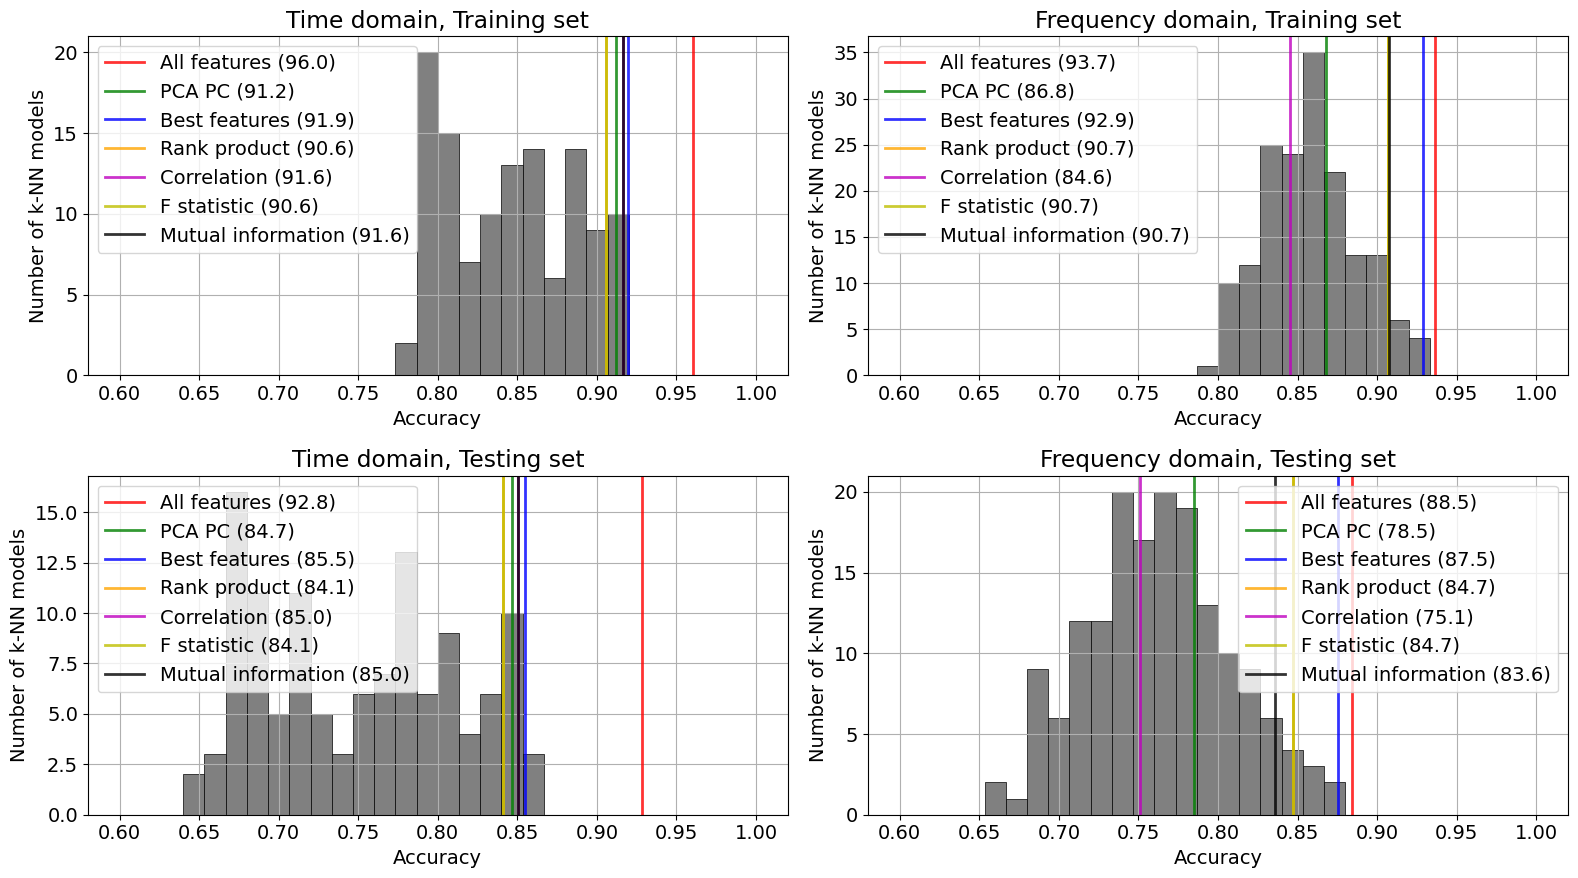
\includegraphics[width=\textwidth]{assets/results/feature-combinations/model-distr-fsel-k5-f3.png}
    \caption{Model distibution with feature selection methods (k = 5, f = 3)}
\end{figure}

% compare dimensions (table)
% Please add the following required packages to your document preamble:
% \usepackage{multirow}
\begin{table}[]
\begin{tabular}{|l|rr|rr|r|l|}
\hline
\multirow{2}{*}{\textbf{Feature set}} & \multicolumn{2}{l|}{\textbf{Accuracy}}                                   & \multicolumn{2}{l|}{\textbf{Percentile}}                                 & \multicolumn{1}{l|}{\multirow{2}{*}{\textbf{Axis}}} & \multirow{2}{*}{\textbf{Best features}} \\ \cline{2-5}
                                      & \multicolumn{1}{l|}{\textbf{Train}} & \multicolumn{1}{l|}{\textbf{Test}} & \multicolumn{1}{l|}{\textbf{Train}} & \multicolumn{1}{l|}{\textbf{Test}} & \multicolumn{1}{l|}{}                               &                                         \\ \hline
All features                          & \multicolumn{1}{r|}{85.56}          & 76.91                              & \multicolumn{1}{r|}{97.58}          & 98.18                              & 1                                                   &                                         \\ \hline
PCA PC                                & \multicolumn{1}{r|}{82.83}          & 72.93                              & \multicolumn{1}{r|}{87.88}          & 86.67                              & 1                                                   &                                         \\ \hline
Best features                         & \multicolumn{1}{r|}{85.97}          & 78.26                              & \multicolumn{1}{r|}{100.00}         & 100.00                             & 1                                                   &                                         \\ \hline
Rank product                          & \multicolumn{1}{r|}{81.93}          & 70.88                              & \multicolumn{1}{r|}{80.00}          & 73.94                              & 1                                                   & roll\_off, roll\_on, flux               \\ \hline
Correlation                           & \multicolumn{1}{r|}{78.85}          & 66.58                              & \multicolumn{1}{r|}{36.36}          & 35.76                              & 1                                                   & roll\_off, kurtosis, skewness           \\ \hline
F statistic                           & \multicolumn{1}{r|}{81.93}          & 70.88                              & \multicolumn{1}{r|}{80.00}          & 73.94                              & 1                                                   & roll\_on, roll\_off, flux               \\ \hline
Mutual information                    & \multicolumn{1}{r|}{81.43}          & 69.91                              & \multicolumn{1}{r|}{73.94}          & 64.85                              & 1                                                   & energy, std, roll\_off                  \\ \hline
All features                          & \multicolumn{1}{r|}{89.34}          & 82.58                              & \multicolumn{1}{r|}{100.00}         & 100.00                             & 3                                                   &                                         \\ \hline
PCA PC                                & \multicolumn{1}{r|}{82.49}          & 71.27                              & \multicolumn{1}{r|}{60.00}          & 57.58                              & 3                                                   &                                         \\ \hline
Best features                         & \multicolumn{1}{r|}{88.55}          & 81.07                              & \multicolumn{1}{r|}{100.00}         & 98.79                              & 3                                                   &                                         \\ \hline
Rank product                          & \multicolumn{1}{r|}{83.84}          & 74.88                              & \multicolumn{1}{r|}{78.18}          & 81.21                              & 3                                                   & flux, roll\_off, std                    \\ \hline
Correlation                           & \multicolumn{1}{r|}{77.58}          & 64.32                              & \multicolumn{1}{r|}{7.27}           & 6.06                               & 3                                                   & flux, skewness, kurtosis                \\ \hline
F statistic                           & \multicolumn{1}{r|}{80.05}          & 68.02                              & \multicolumn{1}{r|}{30.30}          & 30.30                              & 3                                                   & flux, std, skewness                     \\ \hline
Mutual information                    & \multicolumn{1}{r|}{84.17}          & 74.63                              & \multicolumn{1}{r|}{80.00}          & 80.61                              & 3                                                   & roll\_off, roll\_on, flux               \\ \hline
\end{tabular}
\caption{k=5, f=3, bearing=A+B, severity=False, domain=FD}
\end{table}


\begin{table}[]
\begin{tabular}{|l|rr|rr|r|l|}
\hline
\multirow{2}{*}{\textbf{Feature set}} & \multicolumn{2}{l|}{\textbf{Accuracy}}                                   & \multicolumn{2}{l|}{\textbf{Percentile}}                                 & \multicolumn{1}{l|}{\multirow{2}{*}{\textbf{Axis}}} & \multirow{2}{*}{\textbf{Best features}} \\ \cline{2-5}
                                      & \multicolumn{1}{l|}{\textbf{Train}} & \multicolumn{1}{l|}{\textbf{Test}} & \multicolumn{1}{l|}{\textbf{Train}} & \multicolumn{1}{l|}{\textbf{Test}} & \multicolumn{1}{l|}{}                               &                                         \\ \hline
All features                          & \multicolumn{1}{r|}{88.04}          & 81.44                              & \multicolumn{1}{r|}{100.00}         & 100.00                             & 1                                                   &                                         \\ \hline
PCA PC                                & \multicolumn{1}{r|}{84.82}          & 76.42                              & \multicolumn{1}{r|}{95.83}          & 97.50                              & 1                                                   &                                         \\ \hline
Best features                         & \multicolumn{1}{r|}{85.72}          & 77.29                              & \multicolumn{1}{r|}{100.00}         & 100.00                             & 1                                                   &                                         \\ \hline
Rank product                          & \multicolumn{1}{r|}{85.72}          & 77.29                              & \multicolumn{1}{r|}{100.00}         & 100.00                             & 1                                                   & rms, pp, aac                            \\ \hline
Correlation                           & \multicolumn{1}{r|}{83.86}          & 74.92                              & \multicolumn{1}{r|}{85.00}          & 88.33                              & 1                                                   & rms, pp, shape                          \\ \hline
F statistic                           & \multicolumn{1}{r|}{85.72}          & 77.29                              & \multicolumn{1}{r|}{100.00}         & 100.00                             & 1                                                   & rms, pp, aac                            \\ \hline
Mutual information                    & \multicolumn{1}{r|}{85.72}          & 77.29                              & \multicolumn{1}{r|}{100.00}         & 100.00                             & 1                                                   & aac, rms, pp                            \\ \hline
All features                          & \multicolumn{1}{r|}{92.43}          & 88.42                              & \multicolumn{1}{r|}{100.00}         & 100.00                             & 3                                                   &                                         \\ \hline
PCA PC                                & \multicolumn{1}{r|}{87.61}          & 81.66                              & \multicolumn{1}{r|}{96.67}          & 99.17                              & 3                                                   &                                         \\ \hline
Best features                         & \multicolumn{1}{r|}{88.06}          & 80.41                              & \multicolumn{1}{r|}{100.00}         & 98.33                              & 3                                                   &                                         \\ \hline
Rank product                          & \multicolumn{1}{r|}{87.03}          & 79.42                              & \multicolumn{1}{r|}{95.00}          & 94.17                              & 3                                                   & pp, rms, zerocross                      \\ \hline
Correlation                           & \multicolumn{1}{r|}{83.15}          & 73.39                              & \multicolumn{1}{r|}{69.17}          & 68.33                              & 3                                                   & pp, rms, shape                          \\ \hline
F statistic                           & \multicolumn{1}{r|}{86.21}          & 78.26                              & \multicolumn{1}{r|}{88.33}          & 85.83                              & 3                                                   & pp, rms, aac                            \\ \hline
Mutual information                    & \multicolumn{1}{r|}{87.03}          & 79.42                              & \multicolumn{1}{r|}{95.00}          & 94.17                              & 3                                                   & zerocross, rms, pp                      \\ \hline
\end{tabular}
\caption{k=5, f=3, bearing=A+B, severity=False, domain=TD}
\end{table}


\begin{table}[h]
\begin{tabular}{|l|rr|rr|r|l|}
\hline
\multirow{2}{*}{\textbf{Feature set}} & \multicolumn{2}{l|}{\textbf{Accuracy}}                                   & \multicolumn{2}{l|}{\textbf{Percentile}}                                 & \multicolumn{1}{l|}{\multirow{2}{*}{\textbf{Axis}}} & \multirow{2}{*}{\textbf{Best features}} \\ \cline{2-5}
                                      & \multicolumn{1}{l|}{\textbf{Train}} & \multicolumn{1}{l|}{\textbf{Test}} & \multicolumn{1}{l|}{\textbf{Train}} & \multicolumn{1}{l|}{\textbf{Test}} & \multicolumn{1}{l|}{}                               &                                         \\ \hline
All features                          & \multicolumn{1}{r|}{90.82}          & 84.90                              & \multicolumn{1}{r|}{99.39}          & 98.18                              & 1                                                   &                                         \\ \hline
PCA PC                                & \multicolumn{1}{r|}{88.56}          & 82.35                              & \multicolumn{1}{r|}{76.36}          & 76.97                              & 1                                                   &                                         \\ \hline
Best features                         & \multicolumn{1}{r|}{90.89}          & 85.56                              & \multicolumn{1}{r|}{100.00}         & 100.00                             & 1                                                   &                                         \\ \hline
Rank product                          & \multicolumn{1}{r|}{89.65}          & 84.22                              & \multicolumn{1}{r|}{93.94}          & 96.06                              & 1                                                   & entropy, flux, centroid                 \\ \hline
Correlation                           & \multicolumn{1}{r|}{88.48}          & 82.26                              & \multicolumn{1}{r|}{74.55}          & 75.76                              & 1                                                   & entropy, flux, noisiness                \\ \hline
F statistic                           & \multicolumn{1}{r|}{89.65}          & 84.22                              & \multicolumn{1}{r|}{93.94}          & 96.06                              & 1                                                   & entropy, flux, centroid                 \\ \hline
Mutual information                    & \multicolumn{1}{r|}{89.65}          & 84.22                              & \multicolumn{1}{r|}{93.94}          & 96.06                              & 1                                                   & flux, entropy, centroid                 \\ \hline
All features                          & \multicolumn{1}{r|}{92.67}          & 88.19                              & \multicolumn{1}{r|}{100.00}         & 100.00                             & 3                                                   &                                         \\ \hline
PCA PC                                & \multicolumn{1}{r|}{89.37}          & 83.56                              & \multicolumn{1}{r|}{69.09}          & 67.88                              & 3                                                   &                                         \\ \hline
Best features                         & \multicolumn{1}{r|}{91.17}          & 86.97                              & \multicolumn{1}{r|}{100.00}         & 100.00                             & 3                                                   &                                         \\ \hline
Rank product                          & \multicolumn{1}{r|}{88.89}          & 82.69                              & \multicolumn{1}{r|}{55.76}          & 53.94                              & 3                                                   & flux, entropy, skewness                 \\ \hline
Correlation                           & \multicolumn{1}{r|}{88.89}          & 82.69                              & \multicolumn{1}{r|}{55.76}          & 53.94                              & 3                                                   & flux, entropy, skewness                 \\ \hline
F statistic                           & \multicolumn{1}{r|}{88.89}          & 82.69                              & \multicolumn{1}{r|}{55.76}          & 53.94                              & 3                                                   & flux, skewness, entropy                 \\ \hline
Mutual information                    & \multicolumn{1}{r|}{90.15}          & 84.75                              & \multicolumn{1}{r|}{84.24}          & 86.67                              & 3                                                   & roll\_off, flux, roll\_on               \\ \hline
\end{tabular}
\caption{k=5, f=3, bearing=A+B, severity=True, domain=FD}
\end{table}

\begin{table}[]
\begin{tabular}{|l|ll|ll|l|l|}
\hline
\multirow{2}{*}{\textbf{Feature set}} & \multicolumn{2}{l|}{\textbf{Accuracy}}              & \multicolumn{2}{l|}{\textbf{Percentile}}            & \multirow{2}{*}{\textbf{Axis}} & \multirow{2}{*}{\textbf{Best features}} \\ \cline{2-5}
                                      & \multicolumn{1}{l|}{\textbf{Train}} & \textbf{Test} & \multicolumn{1}{l|}{\textbf{Train}} & \textbf{Test} &                                &                                         \\ \hline
All features                          & \multicolumn{1}{l|}{91.56}          & 86.70         & \multicolumn{1}{l|}{100.00}         & 100.00        & 1                              &                                         \\ \hline
PCA PC                                & \multicolumn{1}{l|}{89.82}          & 84.25         & \multicolumn{1}{l|}{93.33}          & 95.00         & 1                              &                                         \\ \hline
Best features                         & \multicolumn{1}{l|}{90.04}          & 84.02         & \multicolumn{1}{l|}{100.00}         & 91.67         & 1                              &                                         \\ \hline
Rank product                          & \multicolumn{1}{l|}{90.00}          & 83.97         & \multicolumn{1}{l|}{99.17}          & 90.00         & 1                              & zerocross, shape, pp                    \\ \hline
Correlation                           & \multicolumn{1}{l|}{89.82}          & 83.96         & \multicolumn{1}{l|}{93.33}          & 88.33         & 1                              & shape, zerocross, rms                   \\ \hline
F statistic                           & \multicolumn{1}{l|}{88.39}          & 82.21         & \multicolumn{1}{l|}{49.17}          & 54.17         & 1                              & pp, rms, shape                          \\ \hline
Mutual information                    & \multicolumn{1}{l|}{89.84}          & 83.67         & \multicolumn{1}{l|}{95.00}          & 83.33         & 1                              & zerocross, aac, rms                     \\ \hline
All features                          & \multicolumn{1}{l|}{93.55}          & 90.50         & \multicolumn{1}{l|}{100.00}         & 100.00        & 3                              &                                         \\ \hline
PCA PC                                & \multicolumn{1}{l|}{91.66}          & 87.31         & \multicolumn{1}{l|}{99.17}          & 99.17         & 3                              &                                         \\ \hline
Best features                         & \multicolumn{1}{l|}{91.91}          & 87.77         & \multicolumn{1}{l|}{100.00}         & 100.00        & 3                              &                                         \\ \hline
Rank product                          & \multicolumn{1}{l|}{91.91}          & 87.77         & \multicolumn{1}{l|}{100.00}         & 100.00        & 3                              & shape, zerocross, rms                   \\ \hline
Correlation                           & \multicolumn{1}{l|}{91.91}          & 87.77         & \multicolumn{1}{l|}{100.00}         & 100.00        & 3                              & shape, rms, zerocross                   \\ \hline
F statistic                           & \multicolumn{1}{l|}{89.27}          & 83.54         & \multicolumn{1}{l|}{73.33}          & 67.50         & 3                              & shape, pp, rms                          \\ \hline
Mutual information                    & \multicolumn{1}{l|}{91.91}          & 87.77         & \multicolumn{1}{l|}{100.00}         & 100.00        & 3                              & zerocross, shape, rms                   \\ \hline
\end{tabular}
\caption{k=5, f=3, bearing=A+B, severity=True, domain=TD}
\end{table}


% compare percentiles
% Feature combinations accuracy
\begin{figure}[h]
    \centering
    \begin{subfigure}[b]{0.48\textwidth}
        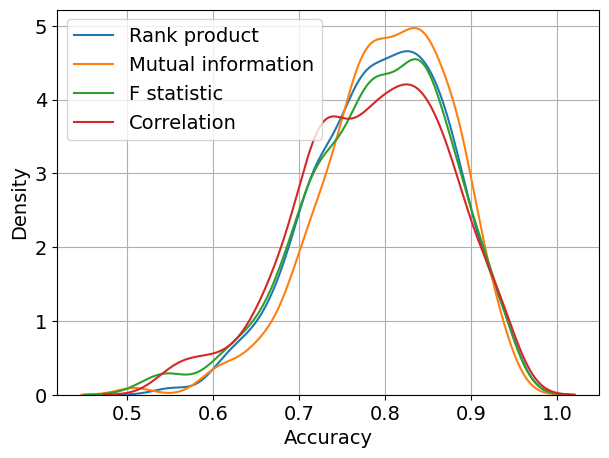
\includegraphics[width=\textwidth]{assets/results/feature-combinations/fsel-accuracy.png}
        \caption{Accuracy}
    \end{subfigure}
    \hfill
    \begin{subfigure}[b]{0.48\textwidth}
        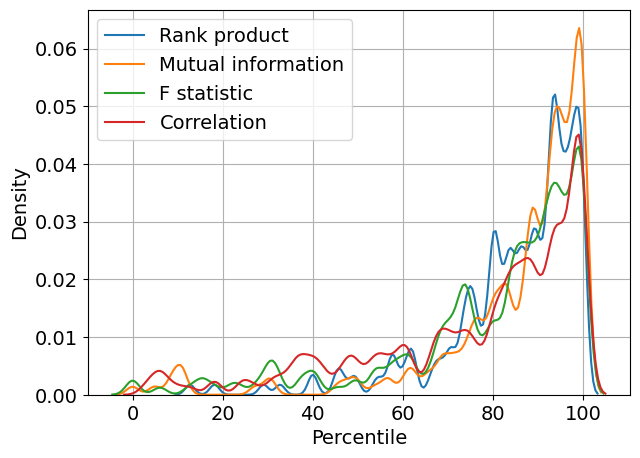
\includegraphics[width=\textwidth]{assets/results/feature-combinations/fsel-percentile.png}
        \caption{Percentile}
    \end{subfigure}
    \caption{Feature selection method choices}
\end{figure}

% In fsel percentile - mention median from notebook for each method - table
\begin{table}[h]
\centering
\begin{tabular}{|l|r|r|}
\hline
\textbf{Method}    & \multicolumn{1}{l|}{\textbf{Median percentile {[}\%{]}}} & \multicolumn{1}{l|}{\textbf{Median accuracy {[}\%{]}}} \\ \hline
Rank product       & 93.94                                                    & 81.84                                                  \\ \hline
Mutual information & 93.33                                                    & 81.33                                                  \\ \hline
F statistic        & 91.01                                                    & 81.26                                                  \\ \hline
Correlation        & 84.11                                                    & 79.25                                                  \\ \hline
\end{tabular}
\end{table}

% Best feature selection methods table (order by best count)
\begin{table}[h]
\centering
\begin{tabular}{|l|r|r|r|}
\hline
                            & \multicolumn{1}{l|}{\textbf{Best in scenarios}} & \multicolumn{1}{l|}{\textbf{Scenarios {[}\%{]}}} & \multicolumn{1}{l|}{\textbf{Mean percentile {[}\%{]}}} \\ \hline
\textbf{Rank product}       & 151                                                     & 69.91                                            & 90.85                                                  \\ \hline
\textbf{Mutual information} & 46                                                      & 21.30                                            & 90.35                                                  \\ \hline
\textbf{Correlation}        & 13                                                      & 6.02                                             & 88.88                                                  \\ \hline
\textbf{F statistic}        & 6                                                       & 2.78                                             & 78.70                                                  \\ \hline
\textbf{$\Sigma$}           & 216                                                     & 100                                       & -                                                      \\ \hline
\end{tabular}
\end{table}

% 2d and 3d plots of best features
\begin{figure}[ht]
    \centering
    \begin{subfigure}[b]{0.48\textwidth}
        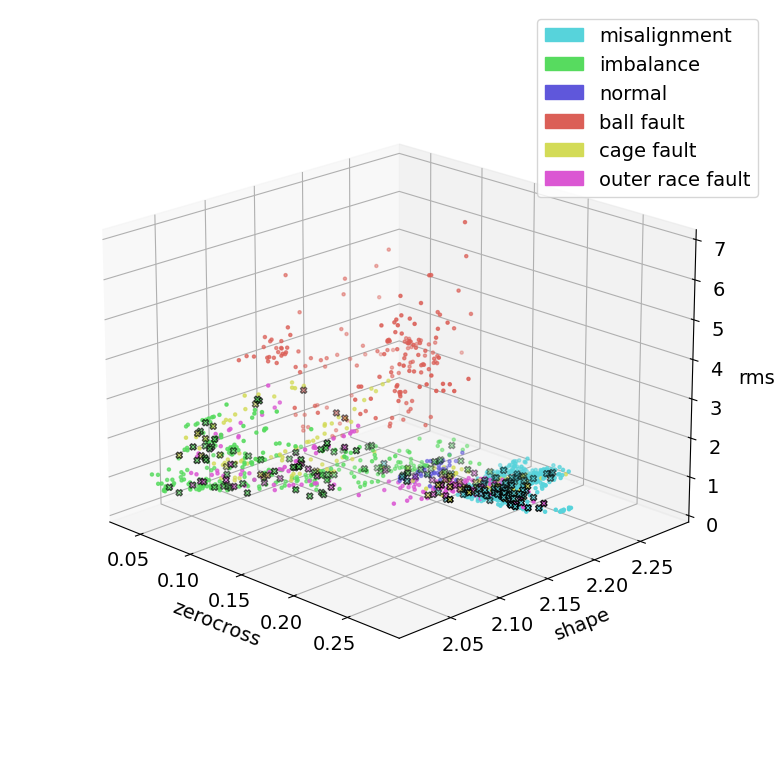
\includegraphics[width=\textwidth]{assets/results/labels/TD.png}
        \caption{Time-domain features}
    \end{subfigure}
    \hfill
    \begin{subfigure}[b]{0.48\textwidth}
        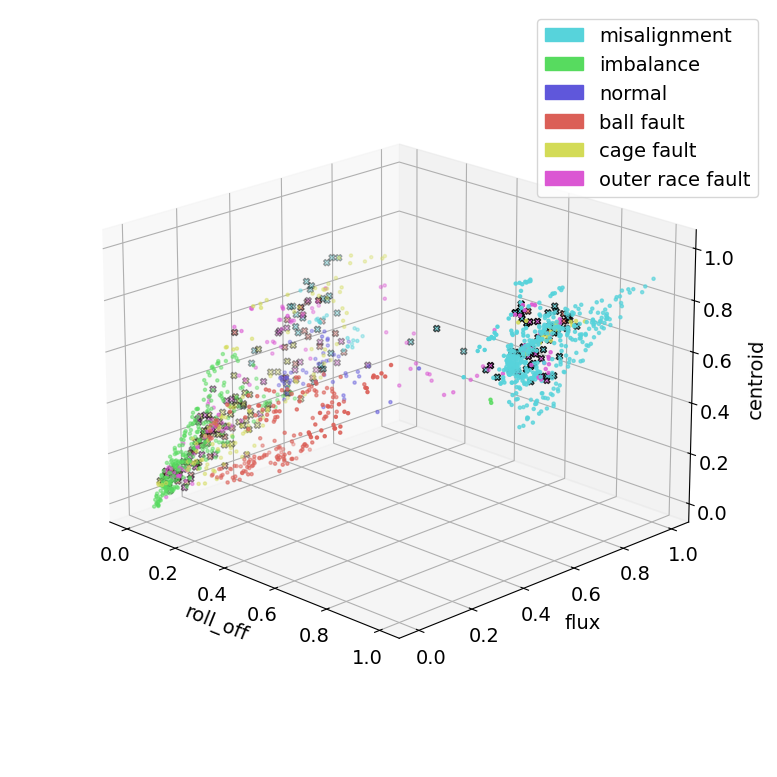
\includegraphics[width=\textwidth]{assets/results/labels/FD.png}
        \caption{Frequency-domain features}
    \end{subfigure}
    \hfill
    \begin{subfigure}[b]{0.48\textwidth}
        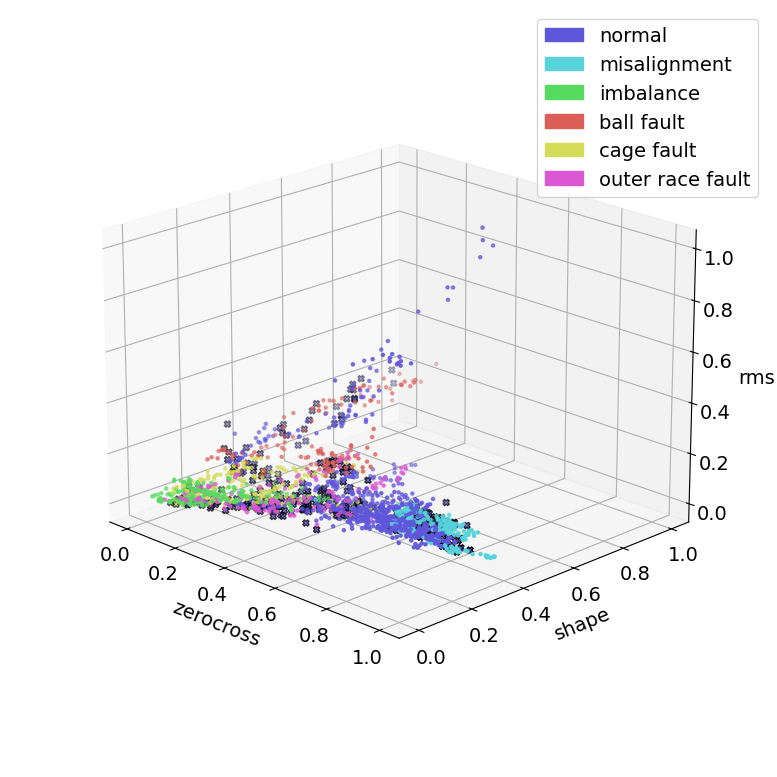
\includegraphics[width=\textwidth]{assets/results/labels/TD-severity.png}
        \caption{Time-domain features (severity)}
    \end{subfigure}
    \hfill
    \begin{subfigure}[b]{0.48\textwidth}
        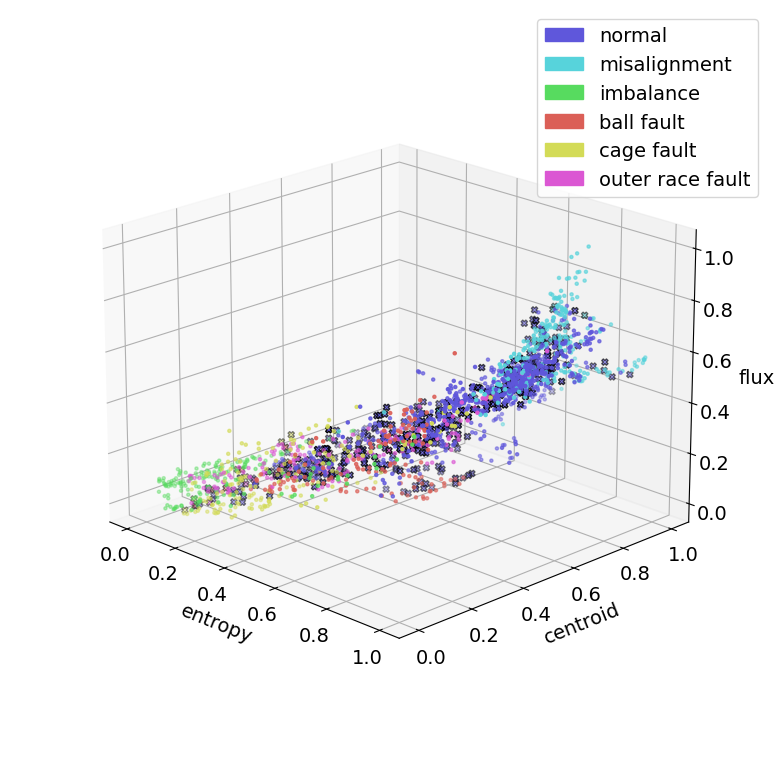
\includegraphics[width=\textwidth]{assets/results/labels/FD-severity.png}
        \caption{Frequency-domain features (severity)}
    \end{subfigure} 
    \caption{3 Best features and their ranges}
\end{figure}

\subsection{Incremental learning}
% Ordering of severity
\begin{figure}[ht]
    \centering
    \begin{subfigure}[b]{0.3\textwidth}
        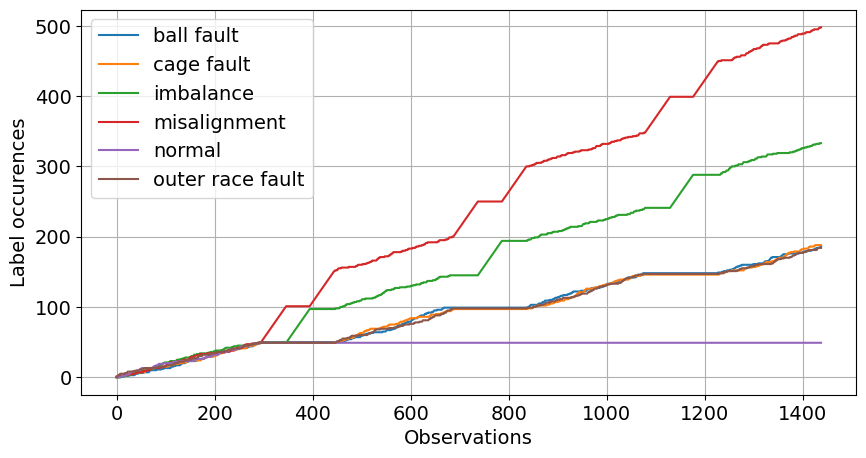
\includegraphics[width=\textwidth]{assets/results/incremental-learning/order-natural.png}
        \caption{Order by raising severity}
    \end{subfigure}
    \hfill
    \begin{subfigure}[b]{0.3\textwidth}
        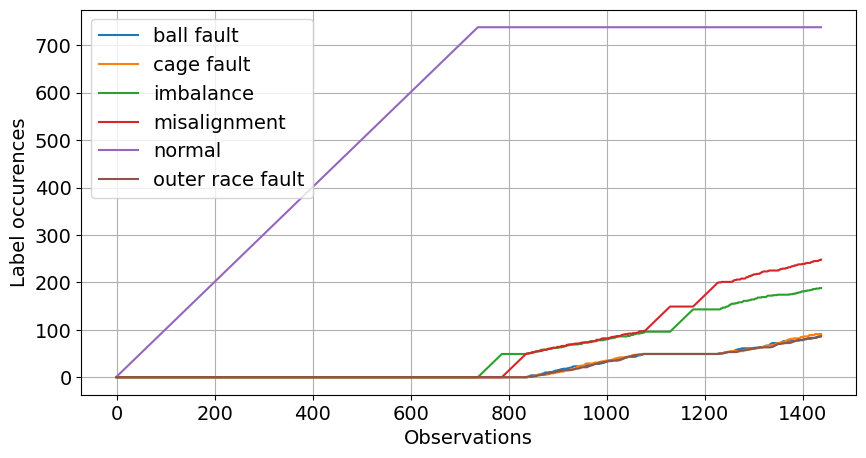
\includegraphics[width=\textwidth]{assets/results/incremental-learning/order-severity.png}
        \caption{Order after relabeing normal class}
    \end{subfigure}
    \hfill
    \begin{subfigure}[b]{0.3\textwidth}
        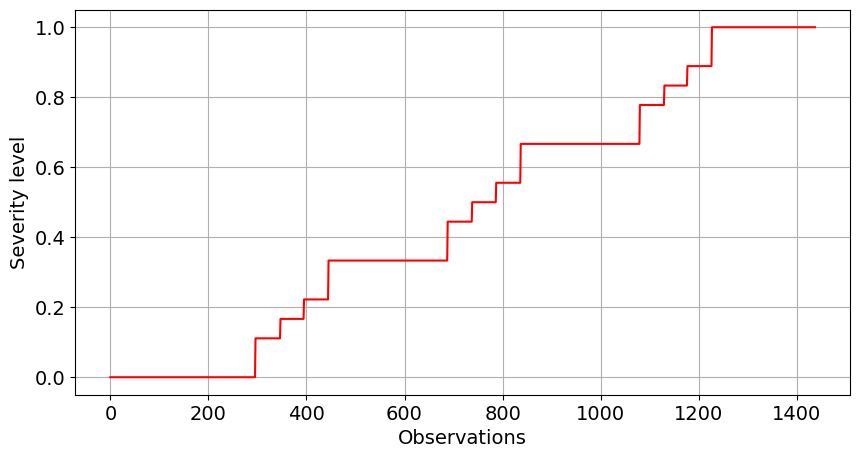
\includegraphics[width=\textwidth]{assets/results/incremental-learning/severity-levels.png}
        \caption{Order of severities}
    \end{subfigure}
    \caption{Ordering of faults}
\end{figure}

% Gradual
\begin{figure}[h]
    \centering
    \begin{subfigure}[b]{0.48\textwidth}
        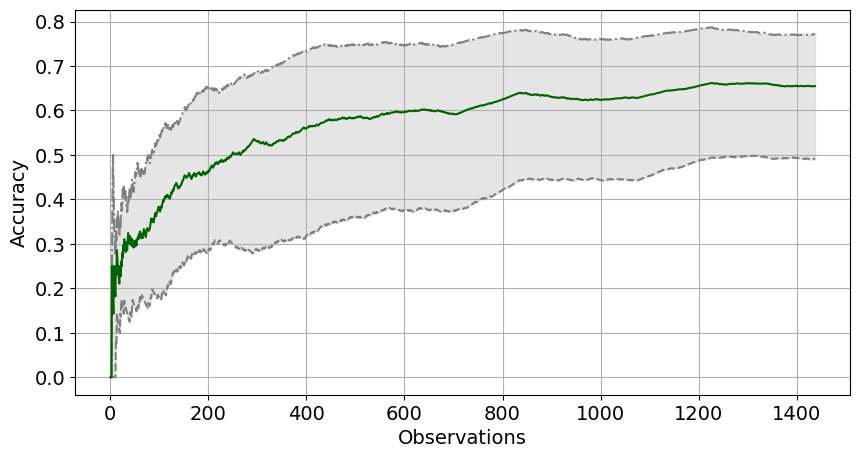
\includegraphics[width=\textwidth]{assets/results/incremental-learning/gradual-TD.png}
        \caption{Time-domain features}
    \end{subfigure}
    \hfill
    \begin{subfigure}[b]{0.48\textwidth}
        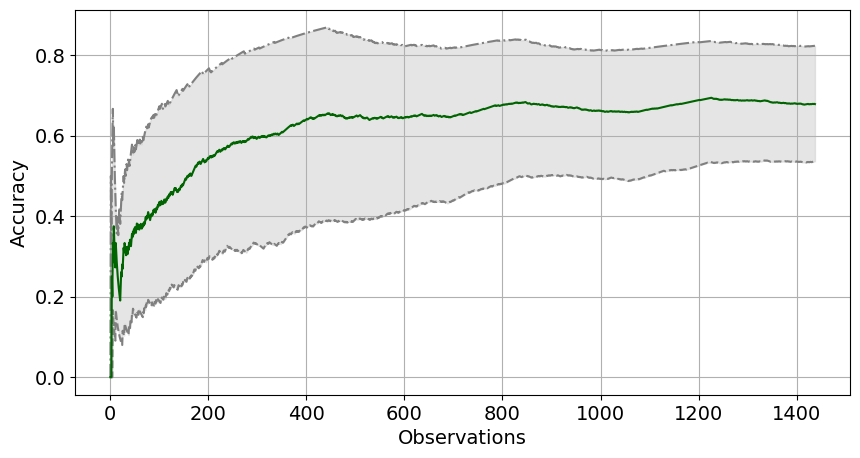
\includegraphics[width=\textwidth]{assets/results/incremental-learning/gradual-FD.png}
        \caption{Frequency-domain features}
    \end{subfigure}
    \hfill
    \begin{subfigure}[b]{0.48\textwidth}
        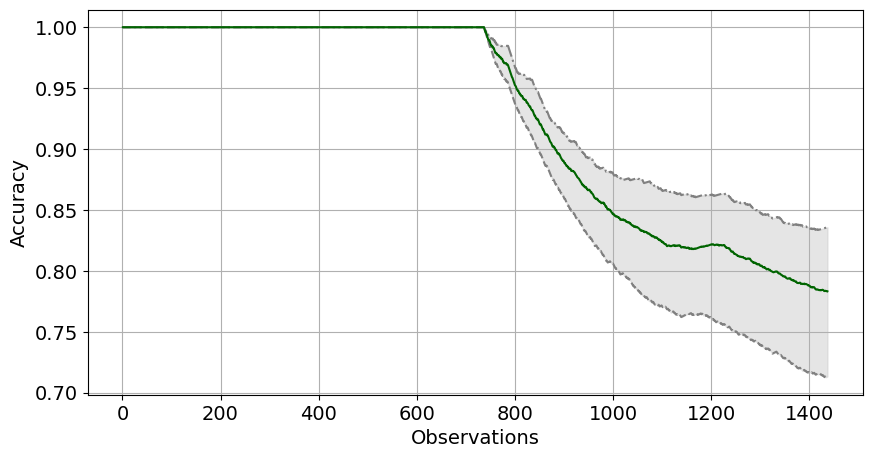
\includegraphics[width=\textwidth]{assets/results/incremental-learning/gradual-TD-severity.png}
        \caption{Time-domain features (severity)}
    \end{subfigure}
    \hfill
    \begin{subfigure}[b]{0.48\textwidth}
        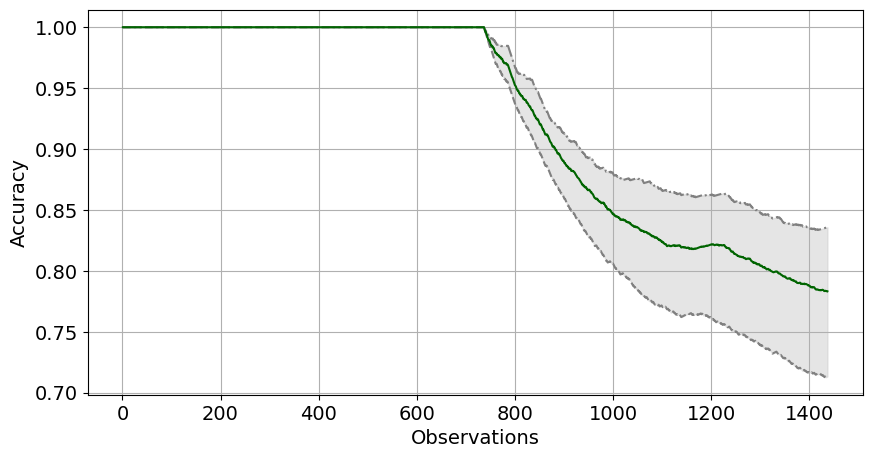
\includegraphics[width=\textwidth]{assets/results/incremental-learning/gradual-TD-severity.png}
        \caption{Frequency-domain features (severity)}
    \end{subfigure} 
    \caption{Gradual learning (window = 1, skip = 0)}
\end{figure}


% Tumbling windows
\begin{figure}[h]
    \centering
    \begin{subfigure}[b]{0.48\textwidth}
        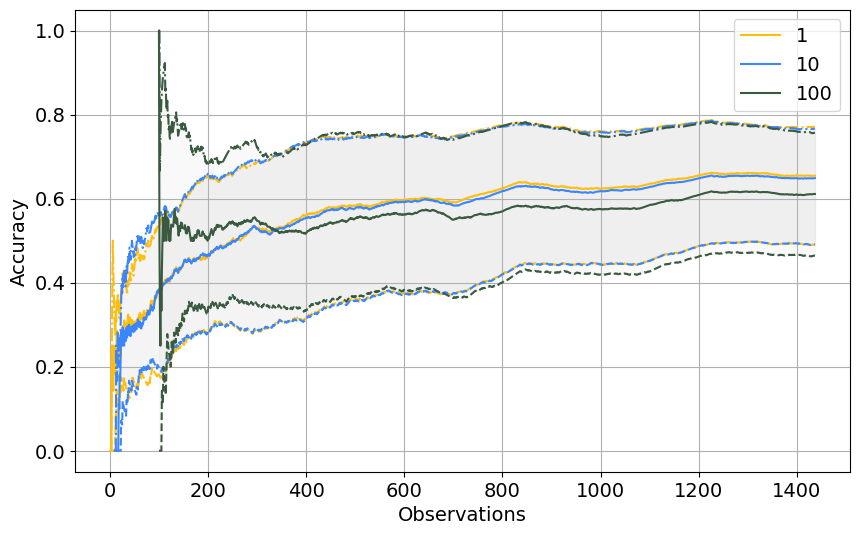
\includegraphics[width=\textwidth]{assets/results/incremental-learning/tumbling-TD.png}
        \caption{Time-domain features}
    \end{subfigure}
    \hfill
    \begin{subfigure}[b]{0.48\textwidth}
        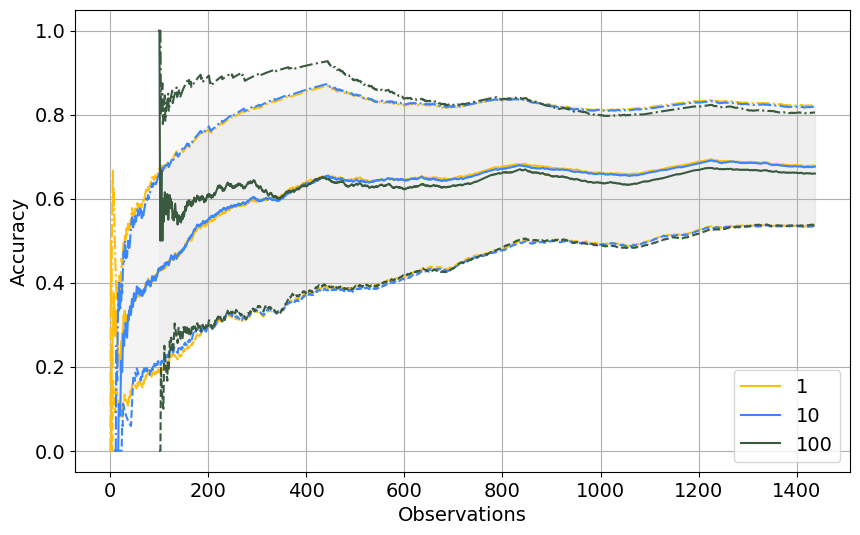
\includegraphics[width=\textwidth]{assets/results/incremental-learning/tumbling-FD.png}
        \caption{Frequency-domain features}
    \end{subfigure}
    \hfill
    \begin{subfigure}[b]{0.48\textwidth}
        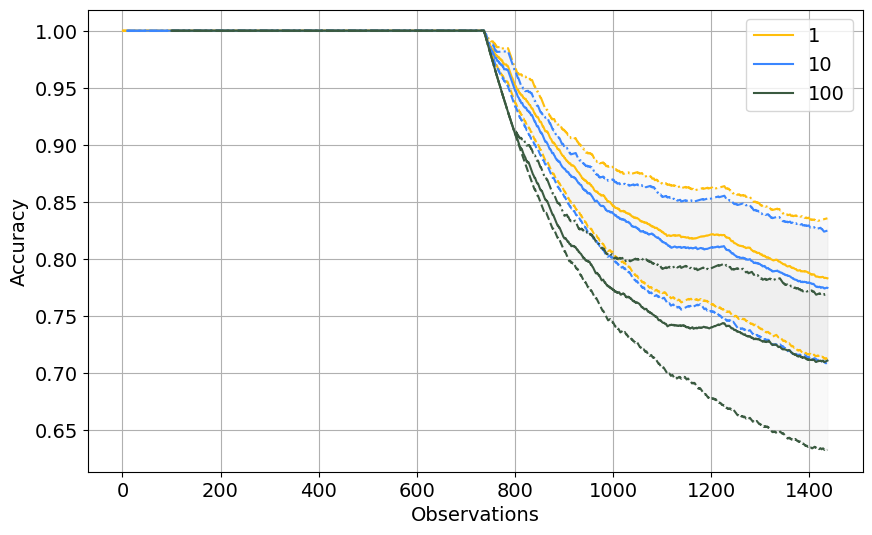
\includegraphics[width=\textwidth]{assets/results/incremental-learning/tumbling-TD-severity.png}
        \caption{Time-domain features (severity)}
    \end{subfigure}
    \hfill
    \begin{subfigure}[b]{0.48\textwidth}
        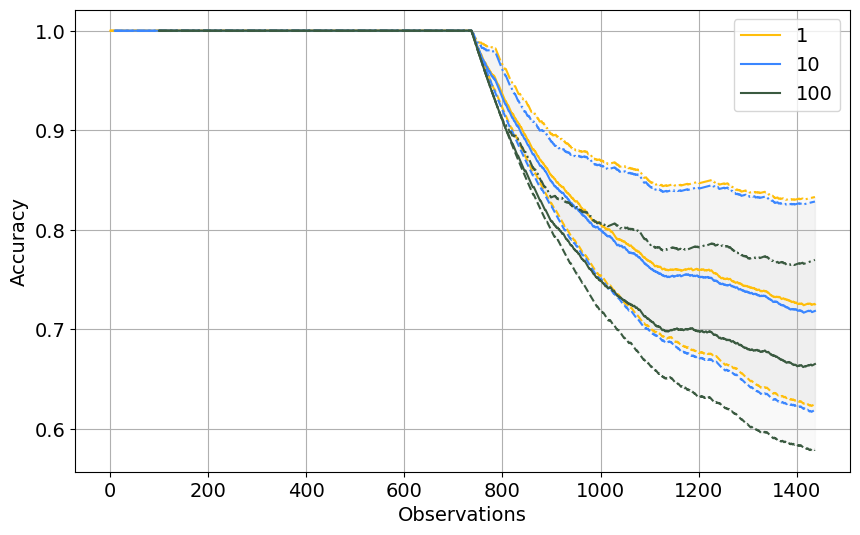
\includegraphics[width=\textwidth]{assets/results/incremental-learning/tumbling-FD-severity.png}
        \caption{Frequency-domain features (severity)}
    \end{subfigure} 
    \caption{Tumbling window in incremental learning}
\end{figure}


% % Label skips and parts of dataset
\begin{figure}[h]
    \centering
    \begin{subfigure}[b]{0.48\textwidth}
        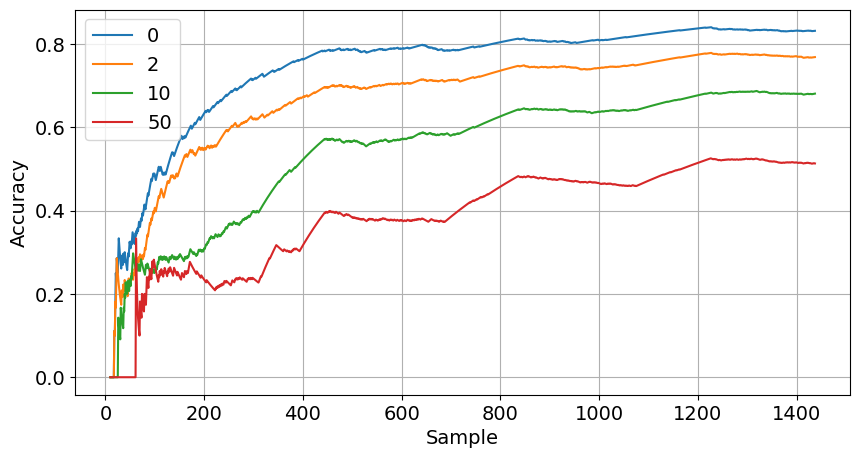
\includegraphics[width=\textwidth]{assets/results/incremental-learning/all-features-TD-skip.png}
        \caption{Time-domain features}
    \end{subfigure}
    \hfill
    \begin{subfigure}[b]{0.48\textwidth}
        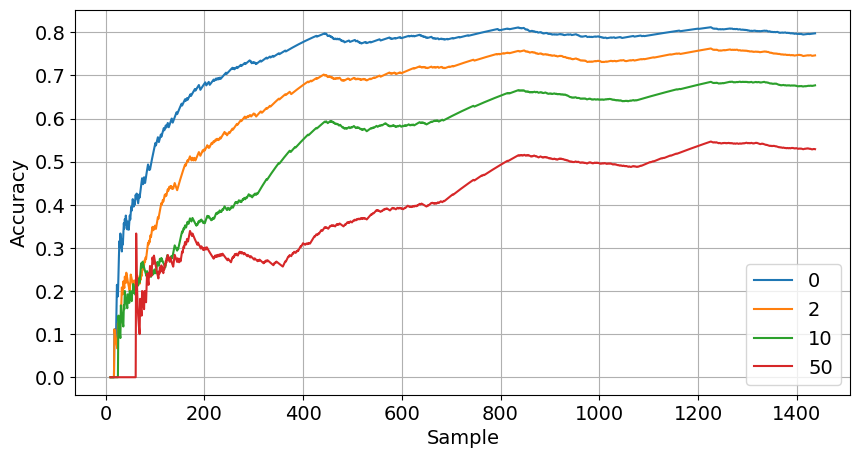
\includegraphics[width=\textwidth]{assets/results/incremental-learning/all-features-FD-skip.png}
        \caption{Frequency-domain features}
    \end{subfigure}
    \hfill
    \begin{subfigure}[b]{0.48\textwidth}
        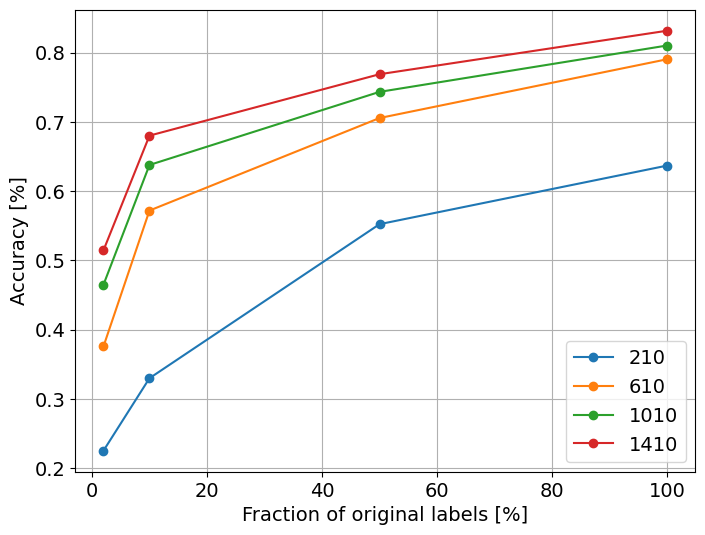
\includegraphics[width=\textwidth]{assets/results/incremental-learning/skip-labels-TD.png}
        \caption{Time-domain features}
    \end{subfigure}
    \hfill
    \begin{subfigure}[b]{0.48\textwidth}
        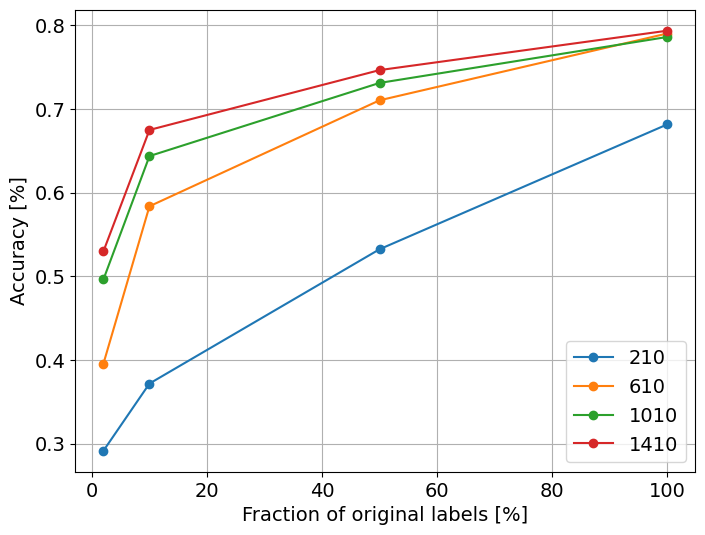
\includegraphics[width=\textwidth]{assets/results/incremental-learning/skip-labels-FD.png}
        \caption{Frequency-domain features}
    \end{subfigure} 
    \caption{Skip labels in incremental learning}
\end{figure}


\begin{figure}[h]
    \centering
    \begin{subfigure}[b]{0.48\textwidth}
        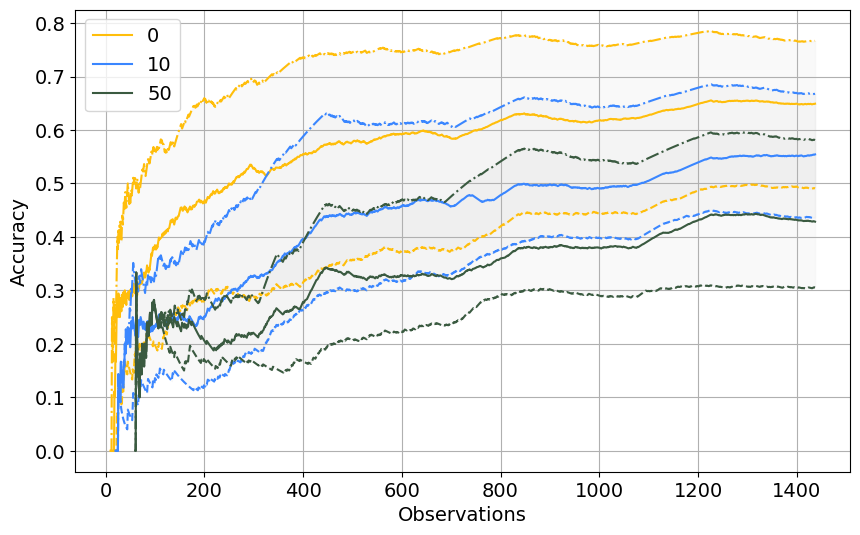
\includegraphics[width=\textwidth]{assets/results/incremental-learning/skip-label-TD.png}
        \caption{Time-domain features}
    \end{subfigure}
    \hfill
    \begin{subfigure}[b]{0.48\textwidth}
        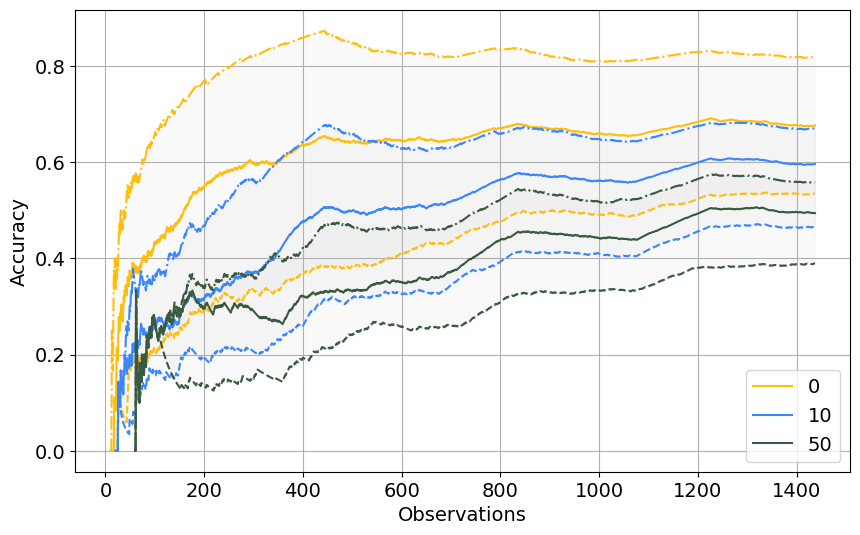
\includegraphics[width=\textwidth]{assets/results/incremental-learning/skip-label-FD.png}
        \caption{Frequency-domain features}
    \end{subfigure}
    \hfill
    \begin{subfigure}[b]{0.48\textwidth}
        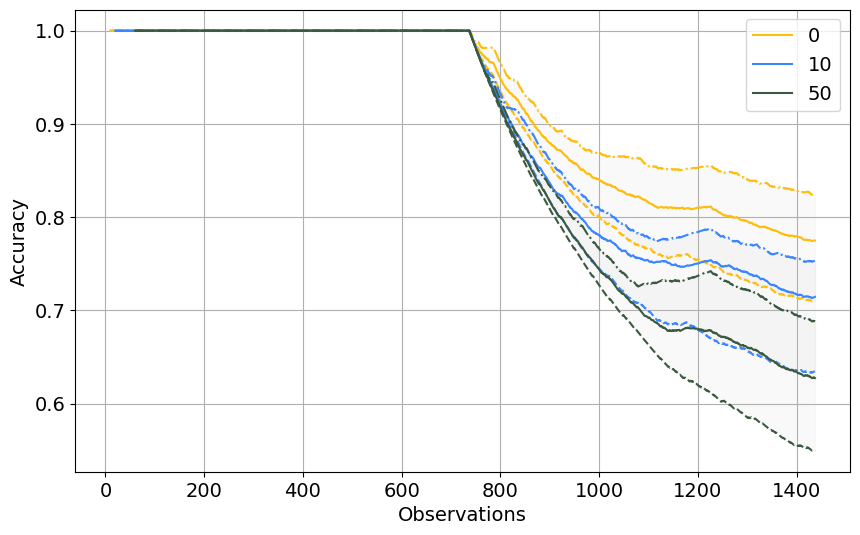
\includegraphics[width=\textwidth]{assets/results/incremental-learning/skip-label-TD-severity.png}
        \caption{Time-domain features (severity)}
    \end{subfigure}
    \hfill
    \begin{subfigure}[b]{0.48\textwidth}
        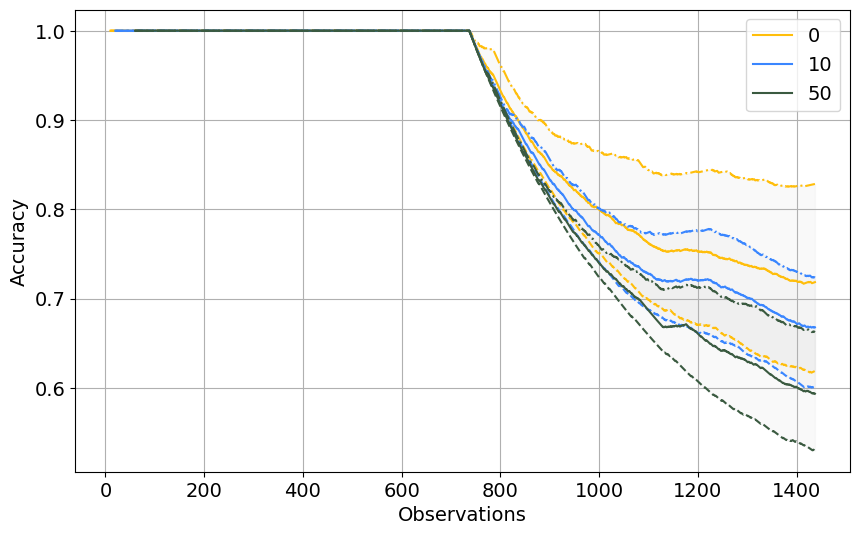
\includegraphics[width=\textwidth]{assets/results/incremental-learning/skip-label-FD-severity.png}
        \caption{Frequency-domain features (severity)}
    \end{subfigure} 
    \caption{Skip labels in incremental learning with different sizes}
\end{figure}




\section{Validation of data logger}
% Validation of firmware on standing fan - speeds
\begin{figure}[ht]
    \centering
    \begin{subfigure}[b]{0.3\textwidth}
        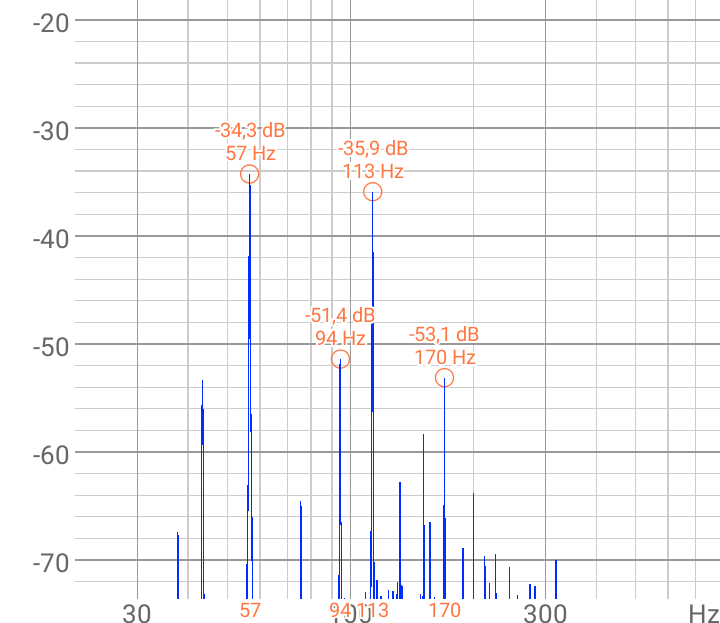
\includegraphics[width=\textwidth]{assets/results/standing-fan/fan-audio-speed-1.png}
        \caption{Speed 1}
    \end{subfigure}
    \hfill
    \begin{subfigure}[b]{0.3\textwidth}
        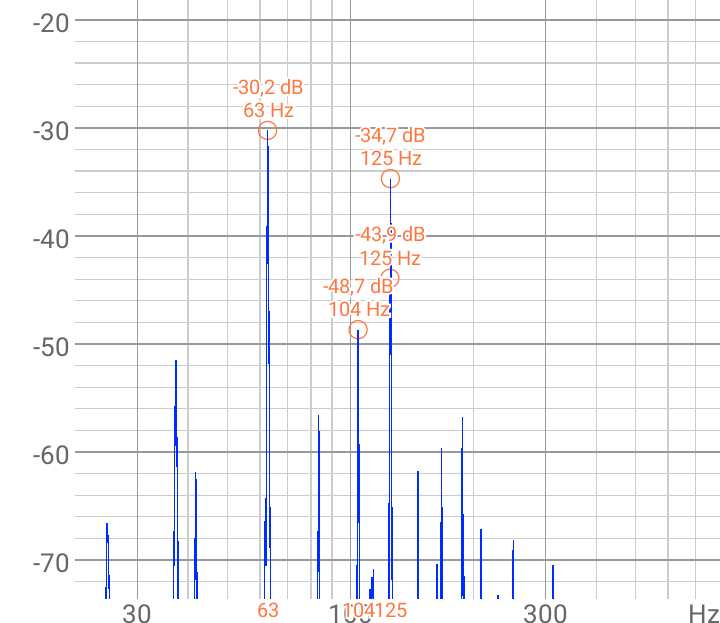
\includegraphics[width=\textwidth]{assets/results/standing-fan/fan-audio-speed-2.png}
        \caption{Speed 2}
    \end{subfigure}
    \hfill
    \begin{subfigure}[b]{0.3\textwidth}
        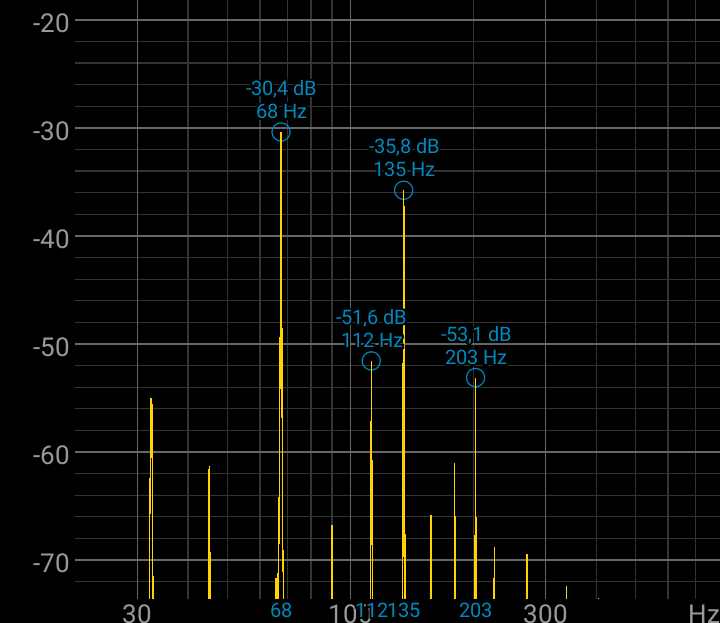
\includegraphics[width=\textwidth]{assets/results/standing-fan/fan-audio-speed-3.png}
        \caption{Speed 3}
    \end{subfigure}
    \caption{Frequency spectrum from sound of standing fan}
\end{figure}

\begin{figure}[ht]
    \centering
    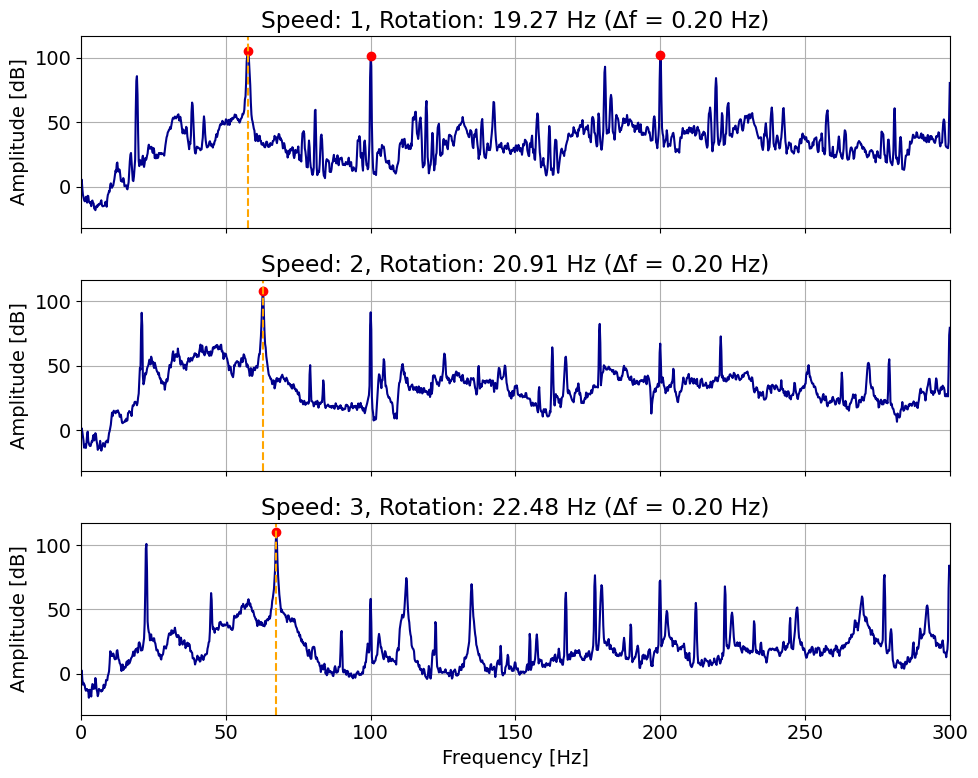
\includegraphics[width=0.5\textwidth]{assets/results/standing-fan/standing-fan-accel.png}
    \caption{Estimation of rotation speed from vibrations}
\end{figure}



\section{Industrial dataset analysis}

\subsection{Feature ranges}
% Amplitude histograms
% Histograms of machinery measurements
\begin{figure}[h]
    \centering
    \begin{subfigure}[b]{0.33\textwidth}
        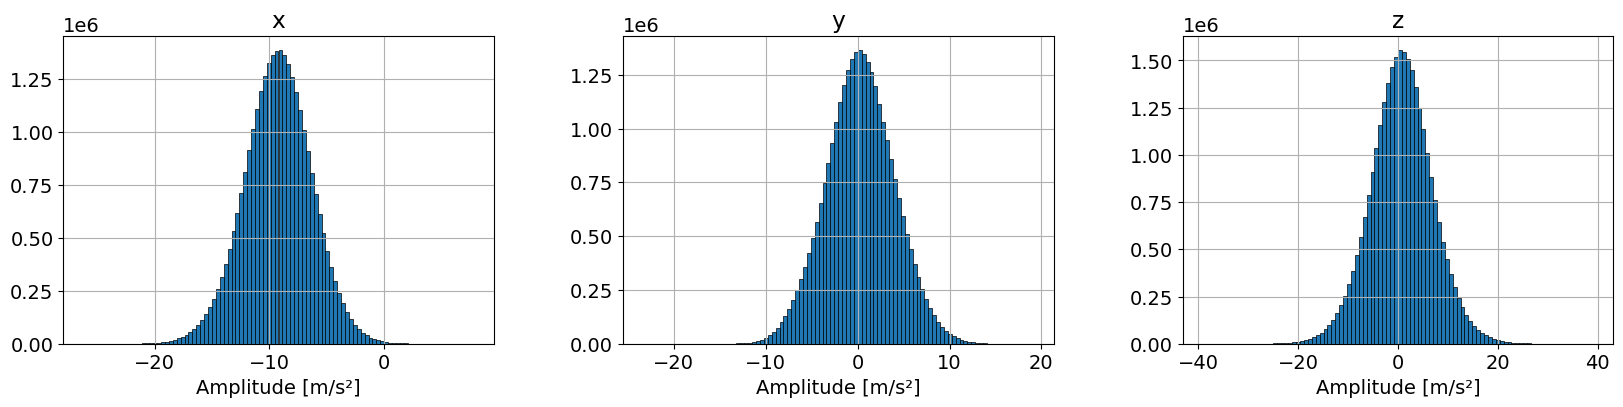
\includegraphics[width=\textwidth]{assets/results/histograms/C1.png}
        \caption{C1}
    \end{subfigure}
    \hfill
    \begin{subfigure}[b]{0.33\textwidth}
        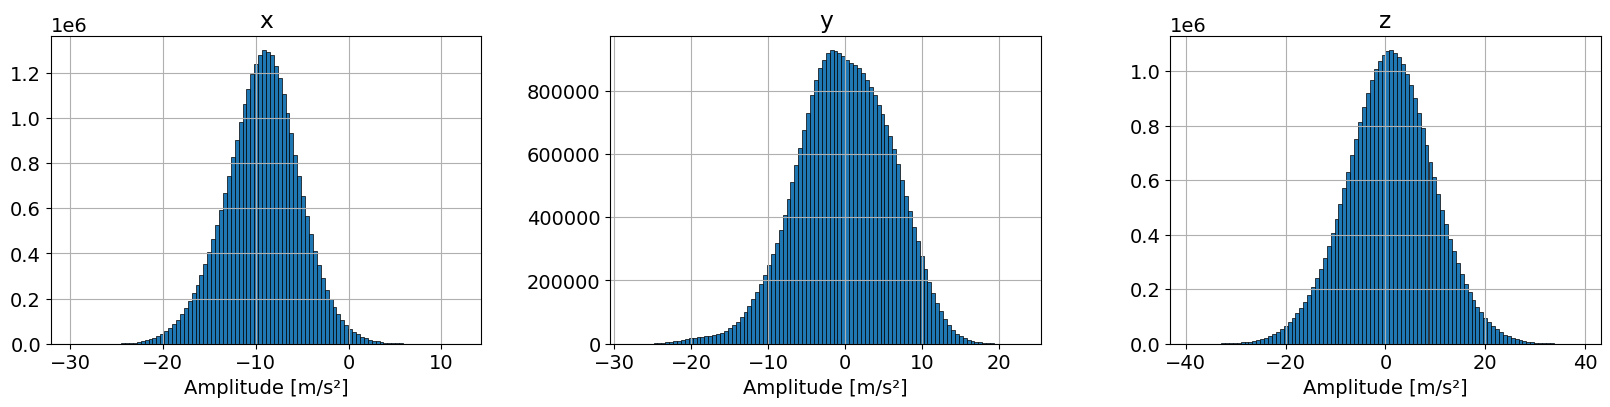
\includegraphics[width=\textwidth]{assets/results/histograms/C2.png}
        \caption{C2}
    \end{subfigure}
    \hfill
    \begin{subfigure}[b]{0.33\textwidth}
        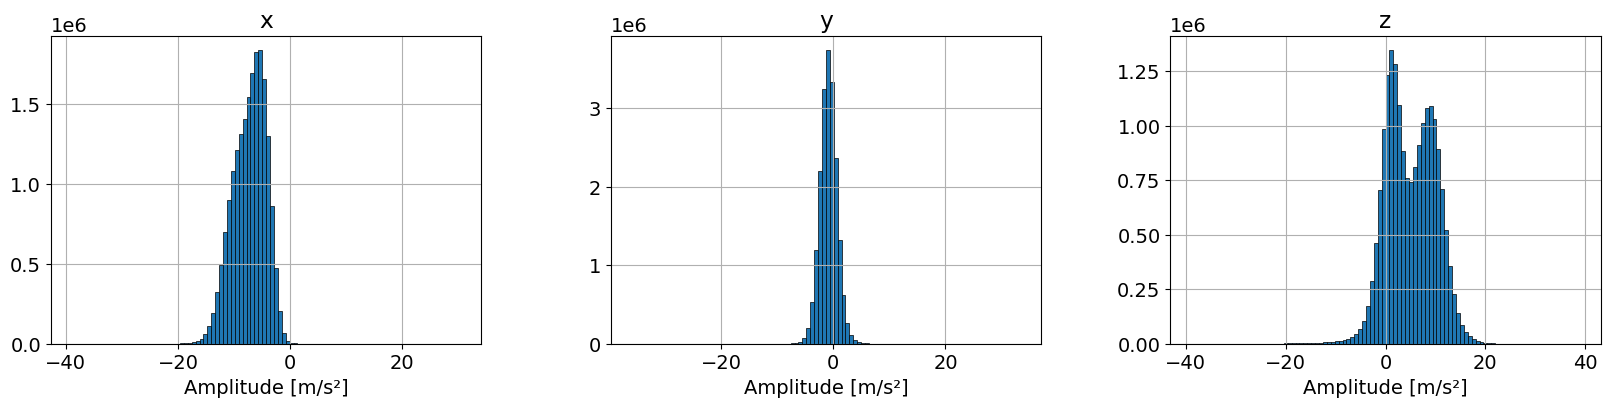
\includegraphics[width=\textwidth]{assets/results/histograms/M1.png}
        \caption{M1}
    \end{subfigure}
    \hfill
    \begin{subfigure}[b]{0.33\textwidth}
        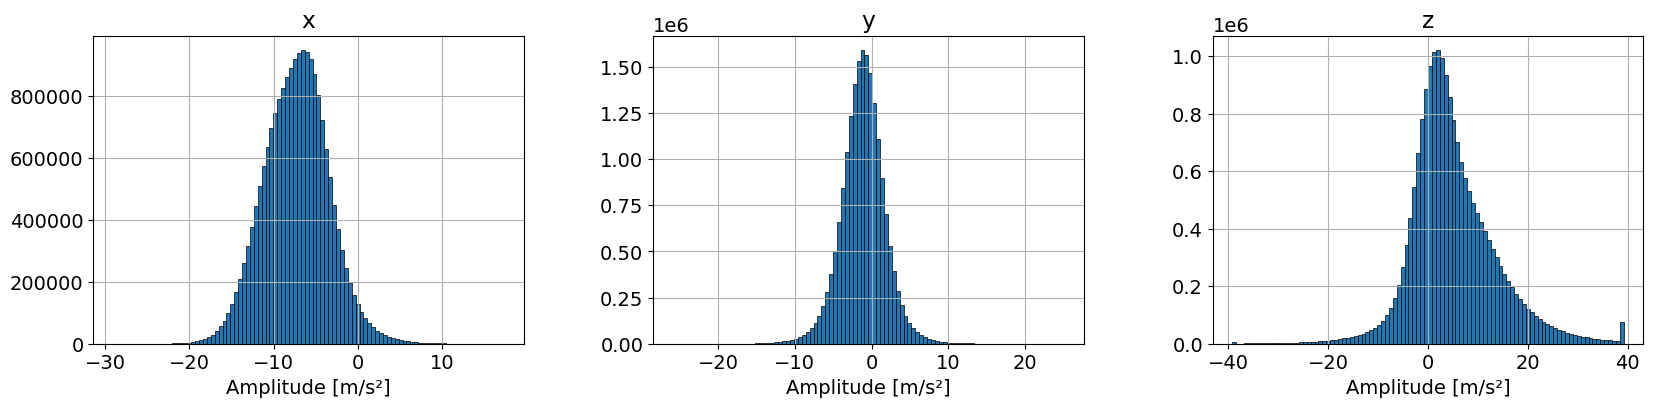
\includegraphics[width=\textwidth]{assets/results/histograms/M2.png}
        \caption{M2}
    \end{subfigure} 
    \hfill
    \begin{subfigure}[b]{0.33\textwidth}
        \includegraphics[width=\textwidth]{assets/results/histograms/M3.png}
        \caption{M3}
    \end{subfigure}
    \hfill
    \begin{subfigure}[b]{0.33\textwidth}
        \includegraphics[width=\textwidth]{assets/results/histograms/P1.png}
        \caption{P1}
    \end{subfigure}
    \hfill
    \begin{subfigure}[b]{0.33\textwidth}
        \includegraphics[width=\textwidth]{assets/results/histograms/P2.png}
        \caption{P2}
    \end{subfigure} 
    \hfill
    \begin{subfigure}[b]{0.33\textwidth}
        \includegraphics[width=\textwidth]{assets/results/histograms/P3.png}
        \caption{P3}
    \end{subfigure} 
    \caption{Histograms}
\end{figure}

% Box plots of features
\begin{figure}[h]
    \centering
    \begin{subfigure}[b]{\textwidth}
        \includegraphics[width=\textwidth]{assets/results/feature-values/pumps-TD-dim-3.png}
        \caption{Time-domain features}
    \end{subfigure}
    \hfill
    \begin{subfigure}[b]{\textwidth}
        \includegraphics[width=\textwidth]{assets/results/feature-values/pumps-FD-dim-3.png}
        \caption{Frequency-domain features}
    \end{subfigure}
    \caption{Feature range in pumps}
\end{figure}

\subsection{Time-frequency waveforms}
\begin{figure}[h]
    \centering
    \begin{subfigure}[b]{0.33\textwidth}
        \includegraphics[width=\textwidth]{assets/results/eda/frequency-spectrum-motors.png}
        \caption{Motors frequency domain}
    \end{subfigure}
    \hfill
    \begin{subfigure}[b]{0.33\textwidth}
        \includegraphics[width=\textwidth]{assets/results/eda/frequency-spectrum-pumps.png}
        \caption{Pumps frequency domain}
    \end{subfigure}
    \hfill
    \begin{subfigure}[b]{0.33\textwidth}
        \includegraphics[width=\textwidth]{assets/results/eda/frequency-spectrum-compressors.png}
        \caption{Compressor frequency domain}
    \end{subfigure} 
    \caption{Frequency domain}
\end{figure}


% Time-frequency spectrum
\begin{figure}[h]
    \centering
    \begin{subfigure}[b]{0.48\textwidth}
        \includegraphics[width=\textwidth]{assets/results/time-frequency-spectrum/K3-z-STFT.png}
        \caption{K3}
    \end{subfigure}
    \hfill
    \begin{subfigure}[b]{0.48\textwidth}
        \includegraphics[width=\textwidth]{assets/results/time-frequency-spectrum/M1-2-z-STFT.png}
        \caption{M1-2}
    \end{subfigure}
    \hfill
    \begin{subfigure}[b]{0.48\textwidth}
        \includegraphics[width=\textwidth]{assets/results/time-frequency-spectrum/P1-3-z-STFT.png}
        \caption{P1-3}
    \end{subfigure}
	\hfill
	\begin{subfigure}[b]{0.48\textwidth}
        \includegraphics[width=\textwidth]{assets/results/time-frequency-spectrum/P3-3-z-STFT.png}
        \caption{P3-3}
    \end{subfigure}
	\hfill
    \begin{subfigure}[b]{0.48\textwidth}
        \includegraphics[width=\textwidth]{assets/results/time-frequency-spectrum/X-P2-Turn-on-Sigma.png}
        \caption{P2-3 turn off with intererence (X-axis)}
    \end{subfigure}
    \caption{Time frequency spectrum}
\end{figure}

% Low frequencies (under 1KHz)

\begin{figure}[h]
    \centering
    \begin{subfigure}[b]{0.48\textwidth}
        \includegraphics[width=\textwidth]{assets/results/time-frequency-spectrum/K3-z-STFT-1kHz.png}
        \caption{K3}
    \end{subfigure}
    \hfill
    \begin{subfigure}[b]{0.48\textwidth}
        \includegraphics[width=\textwidth]{assets/results/time-frequency-spectrum/M1-2-z-STFT-1kHz.png}
        \caption{M1-2}
    \end{subfigure}
    \hfill
    \begin{subfigure}[b]{0.48\textwidth}
        \includegraphics[width=\textwidth]{assets/results/time-frequency-spectrum/P1-3-z-STFT-1kHz.png}
        \caption{P1-3}
    \end{subfigure}
	\hfill
	\begin{subfigure}[b]{0.48\textwidth}
        \includegraphics[width=\textwidth]{assets/results/time-frequency-spectrum/P3-3-z-STFT-1kHz.png}
        \caption{P3-3}
    \end{subfigure}
    \caption{Time frequency spectrum}
\end{figure}


\begin{figure}[h]
    \centering
    \begin{subfigure}[b]{0.48\textwidth}
        \includegraphics[width=\textwidth]{assets/results/time-frequency-spectrum/P1-slow-down.png}
        \caption{Pump P1 turns off}
    \end{subfigure}
    \hfill
    \begin{subfigure}[b]{0.48\textwidth}
        \includegraphics[width=\textwidth]{assets/results/time-frequency-spectrum/P2-speed-up.png}
        \caption{Pump P2 turn on}
    \end{subfigure}
\end{figure}

\subsection{Bearing defect frequencies}
% Domain expert analysis
% Bearing frequencies table
\begin{table}[h]
\centering
\begin{tabular}{|l|r|r|r|}
\hline
\textbf{Placement}     & \multicolumn{1}{l|}{\textbf{Motor \#1}} & \multicolumn{1}{l|}{\textbf{Motor \#2}} & \multicolumn{1}{l|}{\textbf{Pump \#3 \& \#4}} \\ \hline
\textbf{Bearing}       & \multicolumn{1}{l|}{6319-C3}            & \multicolumn{1}{l|}{6324-C3}            & \multicolumn{1}{l|}{6317-2Z}                  \\ \hline
\textbf{$n$}           & 8                                       & 8                                       & 8                                             \\ \hline
\textbf{$f_s$}         & 1493                                    & 1493                                    & 1493                                          \\ \hline
\textbf{$d$ {[}mm{]}}  & 33.12                                   & 41.28                                   & 30.00                                         \\ \hline
\textbf{$D$ {[}mm{]}}  & 147.5                                   & 190.0                                   & 132.5                                         \\ \hline
\textbf{$\beta$}       & 0                                       & 0                                       & 0                                             \\ \hline
\textbf{RPM {[}Hz{]}}  & 24.88                                   & 24.88                                   & 24.88                                         \\ \hline
\textbf{BPFO {[}Hz{]}} & 77.18                                   & 77.91                                   & 77.00                                         \\ \hline
\textbf{BPFI {[}Hz{]}} & 121.88                                  & 121.16                                  & 122.07                                        \\ \hline
\textbf{BSF {[}Hz{]}}  & 58.20                                   & 59.97                                   & 57.77                                         \\ \hline
\textbf{FTF {[}Hz{]}}  & 9.65                                    & 9.74                                    & 9.63                                          \\ \hline
\end{tabular}
\end{table}

% Bearing defect frequencies
\begin{figure}[h]
    \centering
    \begin{subfigure}[b]{0.24\textwidth}
        \includegraphics[width=\textwidth]{assets/results/defects/motors.png}
        \caption{Motors}
    \end{subfigure}
    \hfill
    \begin{subfigure}[b]{0.24\textwidth}
        \includegraphics[width=\textwidth]{assets/results/defects/motors-dB.png}
        \caption{Pumps}
    \end{subfigure}
    \begin{subfigure}[b]{0.24\textwidth}
        \includegraphics[width=\textwidth]{assets/results/defects/pumps.png}
        \caption{Motors}
    \end{subfigure}
    \hfill
    \begin{subfigure}[b]{0.24\textwidth}
        \includegraphics[width=\textwidth]{assets/results/defects/pumps-dB.png}
        \caption{Pumps dB}
    \end{subfigure}
\end{figure}


\subsection{Pump long-term monitoring}
\begin{figure}[h]
    \centering
    \includegraphics[width=0.5\textwidth]{assets/design/sensor/ksb-cloud.jpg}
    \caption{KSB device}
\end{figure}

% Total vibration levels - challange - long-live span (5 years)
\begin{figure}[h]
    \centering
    \begin{subfigure}[b]{0.49\textwidth}
        \includegraphics[width=\textwidth]{assets/results/ksb-cloud/p1.png}
        \caption{Pump P1}
    \end{subfigure}
    \hfill
    \begin{subfigure}[b]{0.49\textwidth}
        \includegraphics[width=\textwidth]{assets/results/ksb-cloud/p2.png}
        \caption{Pump P2}
    \end{subfigure}
    \caption{Vibration levels}
\end{figure}

% Reverse engineer of spectra (low resolution)
\begin{figure}[h]
    \centering
    \includegraphics[width=0.8\textwidth]{assets/results/ksb-cloud/spectrum.png}
    \caption{Frequency spectrum}
\end{figure}


